\chapter{$H^m$ 协调虚单元}

在本章节我们给出任意维数 $d$、任意 $m \in \mathbb{N}$ 的
$H^m$ 协调的虚单元空间,其定义在 $\mathbb R^d$ 中的多面体 $K$
上,满足 $m, d\geq 1$ 且 多形式次数 $k\geq m$。
我们首先介绍了已有的一维和二维情况下的 $H^m$
协调的虚单元,然后推广到任意维的情况。
根据数据空间和 Whitney array 计算出了虚单元空间的维数,证明了自由度的唯一可解性。
给出了虚单元的范数等价性,并将 $H^m$ 
协调虚单元应用到带有低阶项的多重调和方程的求解中。
最后给出数值实验,验证了方法的最优收敛性。

\section{网格假设}
本章中我们考虑 $\mathbb{R}^d$ 中的多面体区域 $\Omega$ 的多面体网格剖分 $\mathcal
T_h$,其满足如下几何条件:
\begin{itemize}
 \item[(A1)] 每个单元$K\in \mathcal T_h$及每个 $r$ 维面 $F$($1\leq r\leq
     d-1$)均为星形区域,且它们的 chunkiness 参数 $\gamma$ 一致有界。

 \item[(A2)] 存在常数$\eta>0$,使得对任意$K\in \mathcal T_h$及$F\in\mathcal
     F^r(K)$($r=1,\cdots, d-1$),满足$h_K\leq\eta h_F$。
\end{itemize}

在本章节中符号 “$\lesssim\cdots$”表示“ $\leq
C\cdots$”,其中常数 $C>0$ 与网格尺寸$h$无关,但可能依赖于网格的 chunkiness 参数、
常数 $\eta$、
多项式次数 $k$、微分阶数 $m$ 以及空间维数$d$。不同不等式中的 $C$ 可取值不同。符号 
$A\eqsim B$ 表示 $A\lesssim B$ 且 $B\lesssim A$。本文中始终假定 $k\geq m$。

\section{$H^m$-协调虚单元}\label{sec:vem}
应用分部积分可以得到如下 Green 公式
\begin{equation}\label{eq:greenidentity}
(\nabla^mv, \nabla^mq)_K=(v, (-\Delta)^mq)_K+\sum_{i=0}^{m-1}(\nabla^{i}v,
\nabla^{i}(-\Delta)^{m-i-1}\partial_{\nnn}q)_{\partial K}.
\end{equation}
对于$v\in H^m(K)$和$q\in H^{2m}(K)$成立。
根据引理 \ref{lemma:nablarv},我们有

\begin{lemma}
设$F\in\mathcal{F}^r(K)$,其中$1\leq r\leq d-1$,$j$为正整数。对于任意光滑函数$v$,成立以下等式:
\begin{equation}\label{eq:20210413}
    \nabla^jv=\sum_{l=0}^j\sum_{\alpha\in \mathbb{T}_r^l} \sum_{\beta\in
    T_{d-r}^{j-l}}\frac{j!}{\alpha!\beta!}\mathrm{sym}(\nnn_F^{\alpha}\otimes
    t_F^{\beta})\frac{\partial^{j}v}{\partial t_F^{\beta}\partial
    \nnn_F^{\alpha}}.
\end{equation} 
% \begin{equation}\label{eq:20210413}
% \nabla^jv=\sum_{\alpha\in A_r, |\alpha|\leq j}\frac{j!}{\alpha!(j-|\alpha|)!}\mathrm{sym}(\nnn_F^{\alpha}\otimes\nabla_F^{j-|\alpha|})\frac{\partial^{|\alpha|}v}{\partial \nnn_F^{\alpha}}。
% \end{equation}
\end{lemma}
\begin{proof}
    根据引理 \ref{lemma:nablarv} 令 $\bt = \{\nnn_{F, 1}, \cdots,
    \nnn_{F, r}, t_{F, 1}, \cdots, t_{F, d-r}\}$,那么 $\bt$ 是 $\mathbb{R}^d$
    的一个标准正交基。代入 \eqref{eq:nablarv} 引理得证。
\end{proof}

\subsection{一维$H^m$协调虚单元}
从一维的虚单元开始,一维情况下多面体 $K$ 是一个区间。自由度$\mathcal N_k^m(K)$选择为
\begin{align}
h_K^jv^{(j)}(\delta) & \quad\forall~\delta\in\mathcal F^{1}(K), \;j=0,1,\cdots,m-1, \label{eq:cfmvem1ddof1}\\
\frac{1}{|K|}(v, q)_K & \quad\forall~q\in\mathbb P_{k-2m}(K), \label{eq:cfmvem1ddof2}
\end{align}
其中$v^{(j)}$是$v$的第$j$阶导数。
取形函数空间为
$$
V_k^m(K):=\{ v\in H^m(K): v^{(2m)}\in \mathbb P_{k-2m}(K)\}=\mathbb P_{\max\{k,2m-1\}}(K).
$$
因此,一维$H^m$协调虚单元恰好是$C^{m-1}$连续的有限元。

\subsection{二维$H^m$协调虚单元}

在二维情况下,多面体 $K$ 是一个多边形。
二维$H^m$协调的虚单元$(K, \mathcal N_k^m(K),
V_k^m(K))$已经在文献
\cite{BeiraoManzini2014,AntoniettiManziniVerani2020,
AntoniettiManziniScacchiVerani2021,BrezziMarini2013}中设计过,这里我们回顾一下。

首先定义一个初步的虚单元空间,以确保虚单元函数 $v$ 到 $\mathbb{P}_k(K)$ 的 $L^2$ 
投影 $Q_k^{K}v$ 可以根据自由度计算,
参考\cite{AhmadAlsaediBrezziMariniEtAl2013}的思路:
\begin{align*}
\widetilde{V}_k^m(K):=\Big\{ v\in H^m(K): &(-\Delta)^mv\in \mathbb P_{k}(K), \\
&\frac{\partial^jv}{\partial \nnn_{e}^j}\Big|_e\in V_{k-j}^{m-j}(e)\quad\forall~e\in\mathcal F^{1}(K),\; j=0,\cdots, m-1\Big\}.    
\end{align*}

显然,$\mathbb P_k(K)\subseteq\widetilde{V}_k^m(K)$,但对于$\frac{\partial^{m-1}v}{\partial \nnn_e^{m-1}}\Big|_e\in\mathbb P_{k-m+1}(e)$,并不一定有$\mathbb P_{k+1}(K)\subseteq\widetilde{V}_k^m(K)$。

\begin{lemma}\label{lem:continuous2d}
对于$v\in\widetilde{V}_k^m(K)$,$\nabla^jv$在$\partial K$上是连续的,其中$j=0,\cdots, m-1$。
\end{lemma}
\begin{proof}
由于$\frac{\partial^{j-\ell}v}{\partial\nnn_e^{j-\ell}}\Big|_e\in \mathbb
P_{\max\{k-j+\ell, 2m-1-2j+2\ell\}}(e)$ 是边 $e\in\mathcal
F^1(K)$的一个多项式。因此根据\eqref{eq:20210413},我们有$\nabla^jv|_e\in\mathbb
P_{\max\{k-j, 2m-1-j\}}(e,\mathbb S_2(j))$。最后,由于$v\in
H^m(K)$,根据\cite{Grisvard1985}中定理1.5.2.3后的注释,我们得到对于$j=0,\cdots,
m-1$,$\nabla^jv\in H^1(K,\mathbb S_2(j))$在$\partial K$上是连续的。
\end{proof}

在$\widetilde{V}_k^m(K)$的定义中,$\frac{\partial^jv}{\partial
\nnn_e^j}\Big|_e\in
V_{k-j}^{m-j}(e)$,所以根据一维的自由度\eqref{eq:cfmvem1ddof1}-\eqref{eq:cfmvem1ddof2}
可知二维情况下的自由度应该包含以下自由度:
\begin{align*}
h_e^i\frac{\partial^i}{\partial t_e^i}\left(\frac{\partial^jv}{\partial \nnn_e^j}\Big|_e\right)(\delta) & \quad\forall~\delta\in\mathcal F^{1}(e), \;i=0,\cdots,m-j-1, \\
\frac{1}{|e|}(\frac{\partial^jv}{\partial \nnn_e^j}, q)_e & \quad\forall~q\in\mathbb P_{k-j-2(m-j)}(e). 
\end{align*}
注意到$\nabla^jv$在$\partial K$上是连续的($j=0,\cdots, m-1$),我们提出了以下
自由度 $\mathcal N_k^m(K)$ 来定义 $\mathbb{R}^2$ 中的 $H^m$ 协调虚单元:
\begin{align}
h_K^j\nabla^{j}v(\delta) & \quad\forall~\delta\in\mathcal F^{2}(K), \;j=0,\cdots,m-1, \label{eq:cfmvem2ddof1}\\
\frac{1}{|e|^{1-j}}(\frac{\partial^jv}{\partial \nnn_e^j}, q)_e & \quad\forall~q\in\mathbb P_{k-2m+j}(e), e\in\mathcal F^{1}(K), \;j=0,\cdots,m-1, \label{eq:cfmvem2ddof2}\\
\frac{1}{|K|}(v, q)_K & \quad\forall~q\in\mathbb P_{k-2m}(K). \label{eq:cfmvem2ddof3}
\end{align}

为了定义形函数空间$V_k^m(K)$,我们还需要一个局部$H^m$投影算子$\Pi_k^K: H^m(K)\to\mathbb P_k(K)$,定义如下:
\begin{align}
(\nabla^m\Pi_k^Kv, \nabla^mq)_K&=(\nabla^mv, \nabla^mq)_K\quad  \forall~q\in \mathbb P_k(K),\label{eq:projlocal2d1}\\
\sum_{\delta\in\mathcal F^{2}(K)}(\nabla^{j}\Pi_k^Kv)(\delta)&=\sum_{\delta\in\mathcal F^{2}(K)}(\nabla^{j}v)(\delta), \quad j=0,\cdots, m-1.\label{eq:projlocal2d2}
\end{align}
根据\cite{AhmadAlsaediBrezziMariniEtAl2013,ChenHuang2020}的思路,定义形函数空间如下:
$$
V_k^m(K):=\{v\in \widetilde{V}_k^m(K): (v-\Pi_k^Kv,
q)_K=0\quad\forall~q\in\mathbb P_{k-2m}^{\perp}(K)\}.
$$
我们有$\mathbb P_k(K)\subseteq V_k^m(K)$,但$\mathbb P_{k+1}(K)\not\subseteq V_k^m(K)$。
因此,我们得到了二维$H^m$协调虚单元$(K, \mathcal N_k^m(K), V_k^m(K))$。

显然我们有:
$$
Q_k^Kv= \Pi_k^Kv + Q_{k-2m}^Kv-Q_{k-2m}^K\Pi_k^Kv.
$$
因此对于 $v\in V_k^m(K)$,$Q_k^Kv$
只使用~\eqref{eq:cfmvem2ddof1}-\eqref{eq:cfmvem2ddof3}中的自由度就可以进行计算。
进一步地,根据分部积分,我们还可以计算出$Q_{k+j}^K(\nabla^jv)$($j=1, \cdots,
m$)。

\subsection{任意维的 $H^m$ 协调虚单元}

下面我们将按照递归的方式构造$k\geq m$且$m\geq1$的任意维度中的$H^m$协调虚单元。

设$K\subset\mathbb R^d$为$d\geq 2$维的多面体。
假设$H^{\ell}$协调虚单元$(F, \mathcal N_{k_{\ell}}^{\ell}(F),
V_{k_{\ell}}^{\ell}(F))$对于$\ell=1,\cdots,
m$且$k_{\ell}\geq\ell$的每个$F\in\mathcal F^r(K)$(其中$r=1,\cdots,
d-1$)都已构造。其中自由度 $\mathcal N_{k_{\ell}}^{\ell}(F)$由以下方式给出:
\begin{align}
h_F^j\nabla_F^{j}v(\delta) & \quad\forall~\delta\in\mathcal F^{d-r}(F), \;j=0,1,\cdots,\ell-1, \label{eq:cfmvemfacesdof1}\\
\frac{h_F^{|\alpha|}}{|e|}(\frac{\partial^{|\alpha|}v}{\partial \nnn_{F,e}^{\alpha}}, q)_e & \quad\forall~q\in\mathbb P_{k_{\ell}-2\ell+|\alpha|}(e), e\in\mathcal F^{s}(F), \; \label{eq:cfmvemfacesdof2}\\
&\quad \quad \quad \alpha\in \mathbb{T}^s_{\leq l-1}, s=1,\cdots,d-r-1,\notag\\
\frac{1}{|F|}(v, q)_F & \quad\forall~q\in\mathbb P_{k_{\ell}-2\ell}(F). \label{eq:cfmvemfacesdof3}
\end{align}
并且假设:
\begin{enumerate}[(i)]
\item \label{item:cfmvemfacesdof1} 
    $\mathbb P_{k_{\ell}}(F)\subseteq V_{k_{\ell}}^{\ell}(F)\subset H^{\ell}(F)$;
\item \label{item:cfmvemfacesdof2} 
    对于任意$v\in V_{k_{\ell}}^{\ell}(F)$,我们有$(\nabla_F^jv)|_{\mathcal
    S_F^s}\in H^{1}(\mathcal S_F^s; \mathbb S_{d-r}(j))$和$(\nabla_F^jv)|_{e}\in
    H^{\ell-j}(e; \mathbb S_{d-r}(j))$,其中$e\in\mathcal
    F^s(F)$,$j=0,1,\cdots,\ell-1$且$s=1,\cdots, d-r-1$;
% \item for any $v\in V_{k_{\ell}}^{\ell}(F)$, $\nabla_F^jv$ is continuous on $\mathcal S_F^1$ for $j=0,1,\cdots, \ell-1$, and $(\nabla_F^jv)|_e$ is a polynomial tensor for each $e\in\mathcal F^{d-r-1}(F)$;
\item \label{item:cfmvemfacesdof3} 
    对于任意$v\in
    V_{k_{\ell}}^{\ell}(F)$,$\frac{\partial^{|\beta|}v}{\partial
    \nnn_{F,e}^{\beta}}\Big|_{e}\in
    V_{k_{\ell}-|\beta|}^{\ell-|\beta|}(e)$对于每个$e\in\mathcal
    F^s(F)$,$\beta\in \mathbb{T}_{\leq\ell-1}^s$且$s=1,\cdots, d-r-1$;
\item \label{item:cfmvemfacesdof4} 
    对于任意$v\in
    V_{k_{\ell}}^{\ell}(F)$,$Q_{k_{\ell}}^F(\nabla_F^jv)$
    只使用形函数空间~\eqref{eq:cfmvemfacesdof1}-\eqref{eq:cfmvemfacesdof3}中的自由度,
    其中 $v\in V_{k_{\ell}}^{\ell}(F)$且$j=0,1,\cdots, \ell$。
\end{enumerate}
假设 (\ref{item:cfmvemfacesdof2}) 受到引理~\ref{lem:continuous2d}的启发。

与二维情况类似,我们首先定义一个初步的虚单元空间
$$
\resizebox{\textwidth}{!}{$
 \begin{aligned}
\widetilde{V}_k^m(K)&:=\big\{ v\in H^m(K):  (-\Delta)^mv\in \mathbb P_{k}(K),  (\nabla^jv)|_{\mathcal S_K^r}\in H^1(\mathcal S_K^r;\mathbb S_{d}(j)) \textrm{ for } 0\leq j\leq m-1, \\
&\quad\;\;\frac{\partial^{|\alpha|}v}{\partial \nnn_F^{\alpha}}\Big|_F\in
V_{k-|\alpha|}^{m-|\alpha|}(F)\quad\forall~F\in\mathcal F^{r}(K), 1\leq r\leq
d-1, \alpha\in \mathbb{T}^r_{\leq m-1}\big\}.
\end{aligned}
$}
$$
根据假设 (\ref{item:cfmvemfacesdof1}),
我们有$\mathbb P_k(K)\subseteq\widetilde{V}_k^m(K)$。
取$v\in\widetilde{V}_k^m(K)$,
应用与引理~\ref{lem:continuous2d}相同的论证,对于每个边$e\in\mathcal F^{d-1}(K)$和$j=0,\cdots, m-1$,我们有$\nabla^jv|_e\in\mathbb P_{\max\{k-j, 2m-1-j\}}(e,\mathbb S_d(j))$,然后由$(\nabla^jv)|_{\mathcal S_K^{d-1}}\in H^1(\mathcal S_K^{d-1};\mathbb S_{d}(j))$可知
$\nabla^jv$在一维骨架$\mathcal S_K^{d-1}$上连续.
对于$F\in\mathcal{F}^r(K)$,其中$1\leq r\leq d-1$,
根据$\widetilde{V}_k^m(K)$的定义和\eqref{eq:20210413},我们有$\nabla^jv|_F\in H^{m-j}(F; \mathbb S_{d}(j))$。

根据 $\frac{\partial^{|\alpha|}v}{\partial \nnn_F^{\alpha}}\Big|_F\in
V_{k-|\alpha|}^{m-|\alpha|}(F)$以及\eqref{eq:cfmvemfacesdof1}-\eqref{eq:cfmvemfacesdof3},
定义如下自由度$\mathcal N_k^m(K)$:
\begin{align}
h_K^j\nabla^{j}v(\delta) & \quad\forall~\delta\in\mathcal F^{d}(K), \;j=0,\cdots,m-1, \label{eq:cfmvemdof1}\\
\frac{h_K^{|\alpha|}}{|F|}(\frac{\partial^{|\alpha|}v}{\partial \nnn_F^{\alpha}}, q)_F & \quad\forall~q\in\mathbb P_{k-2m+|\alpha|}(F), F\in\mathcal F^{r}(K), \; \label{eq:cfmvemdof2}\\
&\quad \quad \alpha\in \mathbb{T}^r_{\leq m-1}, r=1,\cdots,d-1,\notag\\
\frac{1}{|K|}(v, q)_K & \quad\forall~q\in\mathbb P_{k-2m}(K). \label{eq:cfmvemdof3}
\end{align}

为了定义形函数空间$V_k^m(K)$,我们引入了一个局部$H^m$投影算子$\Pi_k^K: H^m(K)\to\mathbb P_k(K)$:给定$v\in H^m(K)$,通过以下等式确定$\Pi_k^Kv\in\mathbb P_k(K)$:
\begin{align}
(\nabla^m\Pi_k^Kv, \nabla^mq)_K&=(\nabla^mv, \nabla^mq)_K\quad  \forall~q\in \mathbb P_k(K),\label{eq:projlocal1}\\
\sum_{\delta\in\mathcal F^{d}(K)}(\nabla^{j}\Pi_k^Kv)(\delta)&=\sum_{\delta\in\mathcal F^{d}(K)}(\nabla^{j}v)(\delta), \quad j=0,\cdots, m-1.\label{eq:projlocal2}
\end{align}
\eqref{eq:projlocal2}中方程的数量是
$
\sum\limits_{j=0}^{m-1}{d-1+j\choose d-1}=\dim\mathbb P_{m-1}(K).
$
我们参考\cite[3.3节引理~3.5]{ChenHuang2020}关于\eqref{eq:projlocal1}-\eqref{eq:projlocal2}的适定性,以及
\begin{equation}\label{eq:localprojprop1}
\Pi_k^Kq=q \quad\forall~q\in\mathbb P_k(K).
\end{equation}
根据假设(\ref{item:cfmvemfacesdof4}),
对于任意 $v\in \tilde{V}_{k}^m(K), F\in\mathcal F^r(K), \alpha\in \mathbb{T}^r_{\leq
m-1}, r=1,\cdots,
d-1$,
$Q_{k-|\alpha|}^F(\nabla_F^{\ell}\frac{\partial^{|\alpha|}}{\nnn_F^{\alpha}}v)$
可通过自由度
\eqref{eq:cfmvemdof1}-\eqref{eq:cfmvemdof2}来计算。
结合 \eqref{eq:20210413} 可知对于 $v \in \tilde{V}_k^m(K)$,$Q_{k-j}^F(\nabla^jv)$可通过使用DoFs
\eqref{eq:cfmvemdof1}-\eqref{eq:cfmvemdof2}来计算。
由\eqref{eq:greenidentity}可知,对于 $v\in \tilde{V}_k^m(K)$,
$\Pi_k^Kv$ 可通过使用自由度
\eqref{eq:cfmvemdof1}-\eqref{eq:cfmvemdof3}来计算。

根据\cite{AhmadAlsaediBrezziMariniEtAl2013,ChenHuang2020}的思路,定义形函数空间
$$
V_k^m(K):=\{v\in \widetilde{V}_k^m(K): (v-\Pi_k^Kv, q)_K=0\quad\forall~q\in\mathbb P_{k-2m}^{\perp}(K)\}.
$$
由\eqref{eq:localprojprop1} 可知 $\mathbb P_k(K)\subseteq V_k^m(K)$。
到此,我们完成了任意维 $H^m$ 协调虚单元 %$(K, \mathcal N_k^m(K), V_k^m(K))$ 
的构建。

\subsection{数据空间和迹}\label{subsec:dataspacetrace}
在本节中,我们将证明自由度 
\eqref{eq:cfmvemdof1}-\eqref{eq:cfmvemdof3}对于局部虚单元空间$V_k^m(K)$是唯一可解的。
其主要困难在于计算 $V_k^m(K)$ 的维度。为此,我们引入数据空间
$$
\mathcal D(\partial K):=\prod_{\delta\in\mathcal F^d(K)}\prod_{j=0}^{m-1}\mathbb
S_d(j) \times \prod_{r=1}^{d-1}\prod_{F\in\mathcal F^r(K)}\prod_{\alpha\in
\mathbb{T}^r_{\leq m-1}}\mathbb P_{k-2m+|\alpha|}(F),
$$
$
\mathcal D(K):=\mathcal D(\partial K)\times\mathbb P_{k-2m}(K)$,以及$\widetilde{\mathcal D}(K):=\mathcal D(\partial K)\times\mathbb P_{k}(K).
$
显然,我们有$\dim\mathcal D(K)=\#\mathcal N_k^m(K)$。
为简便起见,记 $(\ttd_{d}^{\delta, j}, \ttd_{r}^{F, \alpha})\in\mathcal D(\partial K)$表示
\begin{itemize}
\item 对于每个$\delta\in\mathcal F^d(K)$和$j=0,\cdots,m-1$,$\ttd_{d}^{\delta, j}\in\mathbb S_d(j)$;
\item 对于每个$r=1,\cdots, d-1$,$F\in\mathcal F^r(K)$,$\alpha\in \mathbb{T}^r_{\leq
    m-1}$,$\ttd_{r}^{F, \alpha}\in\mathbb P_{k-2m+|\alpha|}(F)$。
\end{itemize}
记$(\ttd_{d}^{\delta, j}, \ttd_{r}^{F, \alpha}, \ttd_0)\in\mathcal
D(K)$表示$(\ttd_{d}^{\delta, j}, \ttd_{r}^{F, \alpha})\in\mathcal D(\partial
K)$,$\ttd_0\in\mathbb P_{k-2m}(K)$。$(\ttd_{d}^{\delta, j}, \ttd_{r}^{F,
\alpha}, \ttd_0)\in\widetilde{\mathcal
D}(K)$的理解方式类似。我们将证明映射$\mathcal D_K: V_k^m(K)\to\mathcal D(K)$ 
$$
\mathcal D_Kv:=\left(\nabla^{j}v(\delta),\; Q_{k-2m+|\alpha|}^F\frac{\partial^{|\alpha|}v}{\partial \nnn_F^{\alpha}},\; (-\Delta)^mv\right) \in \mathcal D(K) \quad\textrm{with}\quad v\in V_k^m(K),
$$
和 $\widetilde{\mathcal D}_K: \widetilde{V}_k^m(K)\to\widetilde{\mathcal D}(K)$
$$
\widetilde{\mathcal D}_Kv:=\bigg(\nabla^{j}v(\delta),\; Q_{k-2m+|\alpha|}^F\frac{\partial^{|\alpha|}v}{\partial \nnn_F^{\alpha}},\; (-\Delta)^mv\bigg) \in \widetilde{\mathcal D}(K) \quad\textrm{with}\quad v\in \widetilde{V}_k^m(K),
$$
都是双射的。引入数据空间的思路可以在\cite{ChenHuang2022}中找到,
类似的自由度元组的想法,在\cite{AntoniettiManziniScacchiVerani2021}中也有提出。

对于一个函数 $v\in H^m(K)$,迹 $\textrm{Tr}\,v$ 定义为:
$$
\mathrm{Tr}\,v = \Big(v|_{\partial K}, \frac{\partial v}{\partial
\nnn_F}\Big|_{\partial K}, \cdots, \frac{\partial^{m-1}v}{\partial
\nnn_F^{m-1}}\Big|_{\partial K}\Big).
$$
显然
$\mathrm{Tr}\,v
\in H^{m-1/2}(\mathcal
F^1(K))\times\cdots\times H^{1/2}(\mathcal F^1(K))$,
其中
$$
H^{s}(\mathcal F^1(K)):=\{v\in L^2(\partial K): v|_F\in H^{s}(F)\;\; \forall~
F\in\mathcal F^1(K)\}.
$$
虽然存在上面的包含关系,但是迹空间 
$\textrm{Tr}\,H^m(K)\neq H^{m-1/2}(\mathcal F^1(K))\times\cdots\times
H^{1/2}(\mathcal
F^1(K))$,这是因为在$\textrm{Tr}\,v$的各个分量之间存在一些兼容性条件
\cite{LambertiProvenzano2020}。
为了呈现在
\cite{Agranovich2007,Agranovich2008,Verchota1990}中对迹空间$\textrm{Tr}\,H^m(K)$
的刻画,我们引入 Whitney array 空间
\begin{align*}
\textrm{WA}(\partial K):=&\,\big\{\{g_{\alpha}\}_{\alpha\in \mathbb{T}^d_{\leq
    m-1}}: g_{\alpha}\in H^1(\partial K)\;\; \forall~\alpha\in
    \mathbb{T}^d_{\leq m-2}, g_{\alpha}\in H^{1/2}(\partial K)\;\;
\forall~\alpha\in \mathbb{T}^d_{|\alpha|= m-1}, \\
&\quad\qquad\quad\quad\quad\quad\;\;\,\textrm{ 且 }\ g_{\alpha} \textrm{ 满足兼容性条件
\eqref{eq:tracecompatiblecond}}\big\},
\end{align*}
其中的兼容性条件为
\begin{equation}\label{eq:tracecompatiblecond}
(\nnn_F)_j\partial_ig_{\alpha}-(\nnn_F)_i\partial_jg_{\alpha}=(\nnn_F)_jg_{\alpha+e_i}-(\nnn_F)_ig_{\alpha+e_j}
\;\;\textrm{ 对于 }F\in\mathcal F^1(K).
\end{equation}
其中 $(\nnn_F)_i=\be_i\cdot\nnn_F$,$\partial_ig_{\alpha}=\be_i\cdot\nabla g_{\alpha}$。

对于$v\in H^m(K)$,很明显我们有 $\{\partial^{\alpha}v|_{\partial K}\}_{\alpha\in
\mathbb{T}^d_{\leq m-1}}\in \textrm{WA}(\partial
K)$,
在这种情况下,\eqref{eq:tracecompatiblecond}
两边的表达式是 $\partial^{\alpha}v$
迹的某个切向导数的两种表示。此外,这样的迹映射是满射的,见如下引理。

\begin{lemma}[见\cite{Agranovich2007}中的定理5, \cite{Agranovich2008}中的定理4和\cite{Verchota1990}中的定理 R(m)]
\label{lem:inversetracethm}
设$K\in\mathbb R^d$是一个多面体。对于每个Whitney array
$\{g_{\alpha}\}_{\alpha\in \mathbb{T}^d_{\leq m-1}}\in \textrm{WA}(\partial K)$,存在一个函数$v\in H^m(K)$满足
$$
\partial^{\alpha}v|_{\partial K}=g_{\alpha}\quad\forall~\alpha\in
\mathbb{T}^d_{\leq m-1}.
$$
此外,存在一个从$\textrm{WA}(\partial K)$到$H^m(K)$的线性有界算子。
\end{lemma}

在接下来的两个引理中,我们将为$\mathcal D(\partial
K)$中的每个数据构造一个Whitney array。

\begin{lemma}\label{lem:dataglue}
给定数据$(\ttd_{d}^{\delta, j}, \ttd_{r}^{F, \alpha})\in\mathcal D(\partial K)$,存在$g_{d}^{\delta,j}\in\mathbb S_d(j)$和$g_{r}^{F,j}\in H^{m-j}(F;\mathbb S_d(j))$,使得对于任意$\delta\in\mathcal F^d(K)$,$F\in\mathcal F^r(K)$,$r=1,\cdots, d-1$和$j=0,\cdots,m-1$,以下条件成立:
\begin{enumerate}[(i)]
\item 对于每个$\delta\in\mathcal F^d(K)$和$j=0,\cdots,m-1$,$g_{d}^{\delta,j}=\ttd_{d}^{\delta, j}$;
\item 对于每个$F\in\mathcal F^r(K)$,$\alpha\in \mathbb{T}^r_{\leq m-1}$和$r=1,\cdots, d-1$,$g_{r}^{F,|\alpha|}:\nnn_F^{\alpha}\in V_{k-|\alpha|}^{m-|\alpha|}(F)$且$Q_{k-2m+|\alpha|}^F(g_{r}^{F,|\alpha|}:\nnn_F^{\alpha})=\ttd_{r}^{F,\alpha}$;
\item 对于每个$F\in\mathcal F^r(K)$,$r=1,\cdots, d-1$和$j=0,\cdots,m-1$,有
\begin{equation}\label{eq:20210425}
    g_{r}^{F,j} = \sum_{l=0}^{j}\sum_{\alpha\in \mathbb{T}^r_{\leq
    l}}\sum_{\beta\in \mathbb{T}^{d-r}_{\leq
    j-l}}\frac{j!}{\alpha!\beta!}\mathrm{sym}(\nnn_F^{\alpha}\otimes t_{F}^{\beta})\frac{\partial^{|\beta|}}{\partial t_{F}^{\beta}}\big(g_{r}^{F,|\alpha|}:\nnn_F^{\alpha}\big);
\end{equation}
\item 对于每个$F\in\mathcal F^ r(K)$,$r=1,\cdots, d-1$,$e\in\mathcal F^s(F)$,$s=1,\cdots, d-r$和$j=0,\cdots,m-1$,$g_{r}^{F,j}|_e=g_{r+s}^{e,j}$。
\end{enumerate}
\end{lemma}

\begin{remark}
我们将在引理~\ref{lem:tidleVkdim}的证明中看到,对于某个 \( v^b\in H^m(K) \),存在 \( g_{r}^{F, j}=\nabla^jv^b|_F \)。在引理~\ref{lem:dataglue}的结论中,对于每个 \( F \in \mathcal{F}^r(K) \) 和 \( |\alpha| \),\( g_{r}^{F,|\alpha|}:\nnn_F^{\alpha}\in V_{k-|\alpha|}^{m-|\alpha|}(F) \) 的定义受到了 \( (\nabla^{|\alpha|}v^b)|_F:\nnn_F^{\alpha}=\frac{\partial^{|\alpha|}v^b}{\partial \nnn_F^{\alpha}}\Big|_F\in V_{k-|\alpha|}^{m-|\alpha|}(F) \) 的启发,这在定义 \( \widetilde{V}_k^m(K) \) 中起着重要作用。对于 自由度 \eqref{eq:cfmvemdof2} 而言,我们有 \( Q_{k-2m+|\alpha|}^F(g_{r}^{F,|\alpha|}:\nnn_F^{\alpha})=\ttd_{r}^{F,\alpha} \),这是基于方程 \eqref{eq:20210413} 的启发。从方程 \eqref{eq:20210425} 我们得到
$$
g_{r}^{F,j}:\mathrm{sym}(\nnn_F^{\alpha}\otimes t_{F}^{\beta}) = \frac{\partial^{|\beta|}}{\partial t_{F}^{\beta}}\big(g_{r}^{F,|\alpha|}:\nnn_F^{\alpha}\big).
$$
\end{remark}

%\begin{proof}
\noindent\textit{引理~\ref{lem:dataglue}的证明}.
首先,对于每个$\delta\in\mathcal F^d(K)$和$j=0,\cdots,m-1$,取$g_{d}^{\delta,j}=\ttd_{d}^{\delta, j}$。
对于每个$e\in\mathcal F^{d-1}(K)$,$\alpha\in \mathbb{T}^{d-1}_{\leq m-1}$,取$v_{d-1}^{e,\alpha}\in V_{k-|\alpha|}^{m-|\alpha|}(e)$,满足以下条件:
\begin{equation*}
\left\{
\begin{aligned}
&\bigg(\frac{\partial^{j}v_{d-1}^{e,\alpha}}{\partial t_e^{j}}\bigg)(\delta)=g_{d}^{\delta, j+|\alpha|}:\mathrm{sym}(\nnn_e^{\alpha}\otimes t_e^j)\quad \forall~\delta\in\mathcal F^1(e), j=0,\cdots,m-|\alpha|-1, \\
&Q_{k-2m+|\alpha|}^e v_{d-1}^{e,\alpha}=\ttd_{d-1}^{e,\alpha}\quad\text{ in } e.
\end{aligned}
\right.
\end{equation*}

对于$j=0,\cdots, m-1$,受到 \eqref{eq:20210413} 的启发,令
$$
g_{d-1}^{e,j} = \sum_{\alpha\in \mathbb{T}^{d-1}_{\leq j}}\frac{j!}{\alpha!(j-|\alpha|)!}\mathrm{sym}(\nnn_e^{\alpha}\otimes t_e^{j-|\alpha|})\bigg(\frac{\partial^{j-|\alpha|}v_{d-1}^{e,\alpha}}{\partial t_e^{j-|\alpha|}}\bigg).
$$
然后对于任意的$\delta\in\mathcal F^1(e)$,我们有
\begin{align*}
    g_{d-1}^{e,j}(\delta)=&\sum_{\alpha\in \mathbb{T}^{d-1}_{\leq j}}\frac{j!}{\alpha!(j-|\alpha|)!}\mathrm{sym}(\nnn_e^{\alpha}\otimes t_e^{j-|\alpha|})\big(g_{d}^{\delta, j}:\mathrm{sym}(\nnn_e^{\alpha}\otimes t_e^{j-|\alpha|})\big)
=g_{d}^{\delta, j}.
\end{align*}
接着有
\begin{align*}
g_{d-1}^{e,|\alpha|}:\nnn_e^{\alpha}=& \sum_{\beta\in \mathbb{T}^{d-1}_{\leq
|\alpha|}}\frac{|\alpha|!}{\beta!(|\alpha|-|\beta|)!}\mathrm{sym}(\nnn_e^{\beta}\otimes t_e^{|\alpha|-|\beta|})\bigg(\frac{\partial^{|\alpha|-|\beta|}v_{d-1}^{e,\beta}}{\partial t_e^{|\alpha|-|\beta|}}\bigg):\nnn_e^{\alpha}\\
=&\, v_{d-1}^{e,\alpha}\in
V_{k-|\alpha|}^{m-|\alpha|}(e)\qquad\qquad\forall~\alpha\in
\mathbb{T}^{d-1}_{\leq m-1}.
\end{align*}
因此我们有
$
Q_{k-2m+|\alpha|}^e(g_{d-1}^{e,|\alpha|}:\nnn_e^{\alpha})=\ttd_{d-1}^{e,\alpha},
$ 以及
$$
g_{d-1}^{e,j} = \sum_{\alpha\in \mathbb{T}^{d-1}_{\leq j}}\frac{j!}{\alpha!(j-|\alpha|)!}\mathrm{sym}(\nnn_e^{\alpha}\otimes t_e^{j-|\alpha|})\frac{\partial^{j-|\alpha|}}{\partial t_e^{j-|\alpha|}}\big(g_{d-1}^{e,|\alpha|}:\nnn_e^{\alpha}\big).
$$

假设对于任意 $e\in\mathcal F^s(K)$,\{$g_{s}^{e,j}\in H^{m-j}(e;\mathbb S_d(j))
\mid s=r+1,\cdots,
d-1$,$j=0,\cdots,m-1$\} 已经找到,
且对于$1\leq r\leq d-2$,满足以下条件
\begin{itemize}
    \item 对于每个$e\in\mathcal F^s(K)$,$\alpha\in \mathbb{T}^s_{\leq m-1}$,$s=r+1,\cdots, d-1$,有$g_{s}^{e,|\alpha|}:\nnn_e^{\alpha}\in V_{k-|\alpha|}^{m-|\alpha|}(e)$ 且 $Q_{k-2m+|\alpha|}^e(g_{s}^{e,|\alpha|}:\nnn_e^{\alpha})=\ttd_{s}^{e,\alpha}$;
\item 对于每个$e\in\mathcal F^s(K)$,$s=r+1,\cdots, d-1$ 和 $j=0,\cdots,m-1$,有
$$
g_{s}^{e,j} = \sum_{l=0}^j\sum_{\alpha \in \mathbb{T}_{l}^s}\sum_{ \beta\in
\mathbb{T}_{j-l}^{d-s}}
\frac{j!}{\alpha!\beta!}\mathrm{sym}(\nnn_e^{\alpha}\otimes
t_{e}^{\beta})\frac{\partial^{|\beta|}}{\partial
t_{e}^{\beta}}\big(g_{s}^{e,|\alpha|}:\nnn_e^{\alpha}\big);
$$
\item 对于每个$e\in\mathcal F^s(K)$,$e'\in\mathcal F^{s'}(e)$,$s=r+1,\cdots, d-1$,$s'=1,\cdots, d-s$,有$g_{s}^{e,j}|_{e'}=g_{s+s'}^{e',j}$。
\end{itemize}
现在考虑每个$F\in\mathcal F^{r}(K)$ 和
$j=1,\cdots,m-1$时$g_{r}^{F,j}$的构建。为此,对于任意$\alpha\in \mathbb{T}^r_{\leq m-1}$,
根据 \eqref{eq:cfmvemfacesdof1}-\eqref{eq:cfmvemfacesdof3},令$v_{r}^{F,\alpha}\in V_{k-|\alpha|}^{m-|\alpha|}(F)$满足:
对于每个 \( F\in\mathcal{F}^{r}(K) \) 和 \( j=1,\cdots,m-1 \),我们将 \( v_{r}^{F,\alpha}\in V_{k-|\alpha|}^{m-|\alpha|}(F) \) 确定为满足以下条件的函数:

$$
\left\{
\begin{aligned}
&\bigg(\frac{\partial^{|\beta|}v_{r}^{F,\alpha}}{\partial\nnn_{F,\delta}^{\beta}}\bigg)(\delta)=g_{d}^{\delta,
|\beta|+|\alpha|}:\mathrm{sym}(\nnn_F^{\alpha}\otimes\nnn_{F,\delta}^{\beta})\quad
\forall~\delta\in\mathcal F^{d-r}(F), \beta\in \mathbb{T}^{d-r}_{\leq
m-|\alpha|-1}, \\
&Q_{k-2m+|\alpha|+|\beta|}^e\bigg(\frac{\partial^{|\beta|}v_{r}^{F,\alpha}}{\partial\nnn_{F,e}^{\beta}}-g_{r+s}^{e, |\beta|+|\alpha|}:\mathrm{sym}(\nnn_F^{\alpha}\otimes\nnn_{F,e}^{\beta})\bigg) = 0\quad \forall~e\in\mathcal F^{s}(F),  \\
&\qquad\qquad\qquad\qquad\qquad\qquad s=1,\cdots,d-r-1,\beta\in
\mathbb{T}^{s}_{\leq m-|\alpha|-1}, \\
&Q_{k-2m+|\alpha|}^Fv_{r}^{F,\alpha}=\ttd_{r}^{F,\alpha}\quad\text{ in } F.
\end{aligned}
\right.
$$
\( V_{k-|\alpha|}^{m-|\alpha|}(F) \) 的自由度 \eqref{eq:cfmvemfacesdof2} 和
\eqref{eq:cfmvemfacesdof3} 可以表示为 \(
h_F^{|\beta|}Q_{k-2m+|\alpha|+|\beta|}^e\frac{\partial^{|\beta|}v}{\partial
\nnn_{F,e}^{\beta}} \) 和 \( Q_{k-2m+|\alpha|}^Fv \),因此 \( v_{r}^{F,\alpha} \)
是良定的。
注意对于 \( e\in\mathcal F^{s}(F) \),有 \(
\frac{\partial^{|\beta|}v_{r}^{F,\alpha}}{\partial\nnn_{F,e}^{\beta}},
g_{r+s}^{e,
|\beta|+|\alpha|}:\mathrm{sym}(\nnn_F^{\alpha}\otimes\nnn_{F,e}^{\beta}) \in
V_{k-|\alpha|-|\beta|}^{m-|\alpha|-|\beta|}(e) \)
,并且它们共享相同的自由度值,因此对于 \( e\in\mathcal F^{s}(F) \) 有

\begin{align}
\label{eq:20210415}
\frac{\partial^{|\beta|}v_{r}^{F,\alpha}}{\partial\nnn_{F,e}^{\beta}}=g_{r+s}^{e, |\beta|+|\alpha|}:\mathrm{sym}(\nnn_F^{\alpha}\otimes\nnn_{F,e}^{\beta})。
\end{align}

对于 \( j=0,\cdots, m-1 \),定义
\begin{align}
\label{eq:20210601}
g_{r}^{F,j} = \sum_{l=0}^{j}\sum_{\alpha\in \mathbb{T}^r_{\leq l}}\sum_{\beta\in
\mathbb{T}^{d-r}_{\leq
j-l}}
\frac{j!}{\alpha!\beta!}\mathrm{sym}(\nnn_F^{\alpha}\otimes t_{F}^{\beta})\bigg(\frac{\partial^{|\beta|}v_{r}^{F,\alpha}}{\partial t_{F}^{\beta}}\bigg)。
\end{align}
那么
$$
g_{r}^{F,|\alpha|}:\nnn_F^{\alpha}=v_{r}^{F,\alpha}\in V_{k-|\alpha|}^{m-|\alpha|}(F),
$$
所以
$$
Q_{k-2m+|\alpha|}^F(g_{r}^{F,|\alpha|}:\nnn_F^{\alpha})=\ttd_{r}^{F,\alpha},
$$
$$
g_{r}^{F,j} = \sum_{l=0}^{j}\sum_{\alpha\in \mathbb{T}^r_{\leq l}}\sum_{\beta\in
\mathbb{T}^{d-r}_{\leq j-l}}
\frac{j!}{\alpha!\beta!}\mathrm{sym}(\nnn_F^{\alpha}\otimes t_{F}^{\beta})\frac{\partial^{|\beta|}}{\partial t_{F}^{\beta}}\big(g_{r}^{F,|\alpha|}:\nnn_F^{\alpha}\big).
$$
对于任意 $e\in\mathcal F^{s}(F), s=1,\cdots,d-r$,根据 \eqref{eq:20210415}-\eqref{eq:20210601} 我们有
\begin{align*}
g_{r}^{F,j}|_e
& = 
\sum_{\alpha\in \mathbb{T}^{r}_{l_0}, \beta\in \mathbb{T}^{s}_{l_1}, \gamma\in
\mathbb{T}^{d-r-s}_{l_2}\atop l_0 + l_1 + l_2 = j}\frac{j!}{\alpha!\beta!\gamma!}\mathrm{sym}(\nnn_F^{\alpha}\otimes \nnn_{F,e}^{\beta}\otimes t_{e}^{\gamma})\frac{\partial^{|\gamma|}}{\partial t_{e}^{\gamma}}\big(g_{r+s}^{e, |\alpha|+|\beta|}:(\nnn_F^{\alpha}\otimes\nnn_{F,e}^{\beta})\big),
\end{align*}
根据假设,它等于 $g_{r+s}^{e,j}$。
最后根据数学归纳法可得到所需结果。
$\hfill\Box$
%\end{proof}

\begin{lemma}\label{lem:datawhitneyarray}
给定数据$(\ttd_{d}^{\delta, j}, \ttd_{r}^{F, \alpha})\in\mathcal D(\partial K)$,
令$g_{1}^{F,j}\in H^{m-j}(F;\mathbb S_d(j))$对于任意$F\in\mathcal
F^1(K)$和$j=0,\cdots,m-1$如引理\ref{lem:dataglue}中定义。
对于每个$\alpha\in \mathbb{T}^d_{\leq m-1}$,通过$g_{\alpha}|_F=g_{1}^{F,|\alpha|}:e^{\alpha}$定义$g_{\alpha}\in L^2(\partial K)$,对于每个$F\in\mathcal F^1(K)$。
那么$\{g_{\alpha}\}_{\alpha\in \mathbb{T}^d_{\leq m-1}}\in \textrm{WA}(\partial K)$。
\end{lemma}
\begin{proof}
通过引理\ref{lem:dataglue}中的(ii)-(iv),对于任意的
$F\in\mathcal
F^1(K)$,以及$\alpha\in \mathbb{T}^d_{\leq m-1}$, 我们有 $g_{\alpha}|_F\in
H^{m-|\alpha|}(F)$ 以及 $g_{\alpha}\in H^1(\partial K)$。

接下来我们检查兼容性条件\eqref{eq:tracecompatiblecond}。
对于 $\ell=1,\cdots, d-1$,根据 \eqref{eq:20210601},
$$
\resizebox{1.0\textwidth}{!}{$
\begin{aligned}
&\quad\; g_{1}^{F,|\alpha|+1}:(e^{\alpha}\otimes t_{F,\ell}) \\
&=\sum_{\beta\in \mathbb{T}^{d-1}_{\leq |\alpha|+1}}\frac{(|\alpha|+1)!}{(|\alpha|+1-|\beta|)!\beta!}\mathrm{sym}(\nnn_F^{|\alpha|+1-|\beta|}\otimes t_{F}^{\beta}):(e^{\alpha}\otimes t_{F,\ell})\frac{\partial^{|\beta|}v_r^{F,|\alpha|+1-|\beta|}}{\partial t_{F}^{\beta}} \\
&=\sum_{\beta\in \mathbb{T}^{d-1}_{\leq |\alpha|}}\frac{|\alpha|!}{(|\alpha|-|\beta|)!\beta!}\mathrm{sym}(\nnn_F^{|\alpha|-|\beta|}\otimes t_{F}^{\beta}):e^{\alpha}\frac{\partial^{|\beta|+1}v_r^{F,|\alpha|-|\beta|}}{\partial t_{F,\ell}\partial t_{F}^{\beta}} = \frac{\partial(g_{1}^{F,|\alpha|}:e^{\alpha})}{\partial t_{F,\ell}}.
\end{aligned}
$}
$$
由于 $e_i=(\nnn_F)_i\nnn_F+\sum\limits_{\ell=1}^{d-1}(t_{F,\ell})_it_{F,\ell}$,我们得到
\begin{equation*}
\resizebox{0.99\textwidth}{!}{$\displaystyle
g_{\alpha+e_i}=g_{1}^{F,|\alpha|+1}:(e^{\alpha}\otimes e_i) =(\nnn_F)_ig_{1}^{F,|\alpha|+1}:(e^{\alpha}\otimes\nnn_F) + \sum_{\ell=1}^{d-1}(t_{F,\ell})_ig_{1}^{F,|\alpha|+1}:(e^{\alpha}\otimes t_{F,\ell}).
$}
\end{equation*}
因此,我们有
\begin{align*}
(\nnn_F)_jg_{\alpha+e_i}-(\nnn_F)_ig_{\alpha+e_j}&=\sum_{\ell=1}^{d-1}\big((\nnn_F)_j(t_{F,\ell})_i-(\nnn_F)_i(t_{F,\ell})_j\big)g_{1}^{F,|\alpha|+1}:(e^{\alpha}\otimes t_{F,\ell}) \\
&=\sum_{\ell=1}^{d-1}\big((\nnn_F)_j(t_{F,\ell})_i-(\nnn_F)_i(t_{F,\ell})_j\big)\frac{\partial g_{\alpha}}{\partial t_{F,\ell}},
\end{align*}
通过计算可知这等于
$(\nnn_F)_j\partial_ig_{\alpha}-(\nnn_F)_i\partial_jg_{\alpha}$,
因此兼容性条件 \eqref{eq:tracecompatiblecond} 成立。
\end{proof}

\subsection{虚单元的唯一可解性}\label{subsec:vemunisolvence}
基于前述引理,现在我们证明任意维 $H^m$ 协调虚单元 $(K, \mathcal N_k^m(K), V_k^m(K))$ 的唯一可解性。
\begin{lemma}\label{lem:tidleVkdim}
映射 $\widetilde{\mathcal D}_K: \widetilde{V}_k^m(K)\to\widetilde{\mathcal D}(K)$ 是满射的。因此
$$
\dim \widetilde{V}_k^m(K)\geq\dim \widetilde{\mathcal D}(K). %\#\mathcal N_k^m(K)+\dim\mathbb P_{k}(K)-\dim \mathbb P_{k-2m}(K)。
$$
\end{lemma}
\begin{proof}
取数据 $(\ttd_{d}^{\delta, j}, \ttd_{r}^{F, \alpha}, \ttd_0)\in\widetilde{\mathcal D}(K)$。
由于 $(\ttd_{d}^{\delta, j}, \ttd_{r}^{F, \alpha})\in\mathcal D(\partial K)$,
根据引理~\ref{lem:datawhitneyarray},
我们可以定义 
$\{g_{\alpha}\}_{\alpha\in \mathbb{T}^d_{\leq m-1}}\in \textrm{WA}(\partial K)$。
根据引理~\ref{lem:inversetracethm},
存在 $v^b\in H^m(K)$,使得对于所有 $\alpha\in \mathbb{T}^d_{\leq m-1}$,都有 $\partial^{\alpha}v^b|_{\partial K}=g_{\alpha}$,也就是说
对于任意 $F\in\mathcal F^1(K)$,
$
\partial^{\alpha}v^b|_F=g_{1}^{F,|\alpha|}:e^{\alpha}$。
这说明对于任意 $F\in\mathcal F^1(K), j=1,\cdots, m-1$,
$\nabla^jv^b|_F=g_{1}^{F, j}$。
根据引理~\ref{lem:dataglue}中的第四点,
我们得到
$$
\nabla^jv^b|_F=g_{r}^{F, j}\quad\forall~F\in\mathcal F^r(K), r=1,\cdots, d,\; j=1,\cdots, m-1.
$$
另一方面,
存在唯一的 $v^0\in H_0^m(K)$ 满足
$
(-\Delta)^mv^0=\ttd_0-(-\Delta)^mv^b.
$
%where $\ttd_0\in \mathbb P_{k}(K)$.
取 $v=v^0+v^b\in H^m(K)$。
我们有 $(-\Delta)^mv=\ttd_0\in\mathbb P_{k}(K)$,并且
\begin{equation}\label{eq:20210527-1}  
\nabla^jv|_F=\nabla^jv^b|_F=g_{r}^{F, j}\quad\forall~F\in\mathcal F^r(K),
r=1,\cdots, d, \; j=1,\cdots, m-1.
\end{equation}
根据上述最后一个等式和引理~\ref{lem:dataglue}中的第四点,我们得到
$(\nabla^jv)|_{\mathcal S_K^r}\in H^1(\mathcal S_K^r;\mathbb S_{d}(j))$,其中 $r=1,\cdots, d-1$,$j=0,\cdots,m-1$。
另外,根据引理~\ref{lem:dataglue}中的第二点,
\begin{equation}\label{eq:20210527-2}  
\frac{\partial^{|\alpha|}v}{\partial
\nnn_F^{\alpha}}\Big|_F=\frac{\partial^{|\alpha|}v^b}{\partial
\nnn_F^{\alpha}}\Big|_F=g_{r}^{F, |\alpha|}:\nnn_F^{\alpha}\in
V_{k-|\alpha|}^{m-|\alpha|}(F).
\end{equation}
对于任意 $F\in\mathcal F^{r}(K)$,$r=1,\cdots, d-1$,$\alpha\in
\mathbb{T}^r_{\leq m-1}$ 都成立。
因此,
$v\in \widetilde{V}_k^m(K)$。根据\eqref{eq:20210527-1}-\eqref{eq:20210527-2}、引理~\ref{lem:dataglue}中的第一和第二点,我们得到 $\widetilde{\mathcal D}_Kv=(\ttd_{d}^{\delta, j}, \ttd_{r}^{F, \alpha}, \ttd_0)$。
\end{proof}
%This ends the proof.

\begin{lemma}\label{lem:tildevemunisolvence}
以下的自由度 $\widetilde{\mathcal N}_k^m(K)$
\begin{align*}
h_K^j\nabla^{j}v(\delta) & \quad\forall~\delta\in\mathcal F^{d}(K), \;j=0,1,\cdots,m-1, \\
\frac{h_K^{|\alpha|}}{|F|}(\frac{\partial^{|\alpha|}v}{\partial \nnn_F^{\alpha}}, q)_F & \quad\forall~q\in\mathbb P_{k-2m+|\alpha|}(F), F\in\mathcal F^{r}(K), \;r=1,\cdots,d-1, \\
&\quad \quad \alpha\in \mathbb{T}^r_{\leq m-1}, \\
\frac{1}{|K|}(v, q)_K & \quad\forall~q\in\mathbb P_{k}(K).
\end{align*}
对于局部虚单元空间 $\widetilde{V}_k^m(K)$ 是唯一可解的。
因此,映射 $\widetilde{\mathcal D}_K: \widetilde{V}_k^m(K)\to\widetilde{\mathcal D}(K)$ 是双射。
\end{lemma}
\begin{proof}
由引理~\ref{lem:tidleVkdim},我们有 $\dim\widetilde{V}_k^m(K)\geq\#\widetilde{\mathcal N}_k^m(K)$。假设 $v\in\widetilde{V}_k^m(K)$ 且 $\widetilde{\mathcal N}_k^m(K)$ 中的所有自由度都为零。根据 $\widetilde{V}_k^m(K)$ 的递归定义,由于 $\widetilde{\mathcal N}_k^m(K)$ 中边界上的自由度为零,可知 $v\in H_0^m(K)$。利用分部积分,我们有 $(-\Delta)^mv|_K\in\mathbb P_k(K)$,因此
$
\|\nabla^mv\|_{0,K}^2=(v, (-\Delta)^mv)_K=0。
$
这意味着 $v=0$。

\end{proof}

\begin{lemma}
自由度~\eqref{eq:cfmvemdof1}-\eqref{eq:cfmvemdof3},即 $\mathcal N_k^m(K)$,对于局部虚单元空间 $V_k^m(K)$ 是唯一可解的。
因此,映射 $\mathcal D_K: V_k^m(K)\to\mathcal D(K)$ 是双射。
\end{lemma}
\begin{proof}
根据 $V_k^m(K)$ 的维数定义,我们有 $\dim V_k^m(K)\geq \#\mathcal N_k^m(K)$。
假设 $v\in V_k^m(K)$ 且自由度~\eqref{eq:cfmvemdof1}-\eqref{eq:cfmvemdof3} 都为零。
注意到 $\Pi_k^Kv=0$。因此对于所有的 $q\in\mathbb P_k(K)$,都有
$
(v, q)_K=0,
$
这与引理~\ref{lem:tildevemunisolvence} 结合起来得出 $v=0$。
\end{proof}

与二维情况类似,我们有
\begin{equation}\label{eq:QkKrepresent}
    Q_k^Kv= \Pi_k^Kv + Q_{k-2m}^Kv-Q_{k-2m}^K\Pi_k^Kv\quad\forall~v\in V_k^m(K).
\end{equation}
因此,对于任意 $v\in V_k^m(K)$,
$Q_k^Kv$ 可以仅使用自由度~\eqref{eq:cfmvemdof1}-\eqref{eq:cfmvemdof3}
来计算,进而可得 $Q_{k}^K(\nabla^jv), j=1, \cdots, m$, 
可以仅使用自由度~\eqref{eq:cfmvemdof1}-\eqref{eq:cfmvemdof3} 来计算。根据
\eqref{eq:QkKrepresent},我们有
\begin{equation}\label{eq:QkKrepresentkerpi}
    Q_k^Kv= Q_{k-2m}^Kv\quad\forall~v\in \ker(\Pi_k^K)\cap V_k^m(K),
\end{equation}
其中 $\ker(\Pi_k^K)\cap V_{k}^{m}(K):=\{v\in V_{k}^{m}(K): \Pi_k^Kv=0\}$。

%我们参考了文献 \cite{BeiraodaVeigaDassiRusso2020} 中三维情况下的 $H^2$-conforming 虚单元方法。
\begin{remark}\rm
对于最低次数情况$k=m$,自由度 \eqref{eq:cfmvemdof2}-\eqref{eq:cfmvemdof3}
个数为 0
,$\mathcal N_k^m(K)$ 将简化为
$$
h_K^j\nabla^{j}v(\delta) \quad\forall~\delta\in\mathcal F^{d}(K), \;j=0,1,\cdots,m-1.
$$
\end{remark}

\begin{remark}\rm
当$k=m$且$K\subset\mathbb R^d$为单纯形时,
$$
\dim V_k^m(K)=(d+1)\dim\mathbb P_{m-1}(K).
$$
作为对比,在文献\cite{HuLinWu2021,ChenHuang2021Cmgeodecomp}中最低次数的 $H^m$ 
协调有限元的维度为$\dim \mathbb P_{2^d(m-1)+1}(K)$,远远大于$\dim V_k^m(K)$。
\end{remark}

\section{逆不等式与范数等价性}\label{sec:invnorm}

在本节中,我们将通过数学归纳推导虚单元$(K, \mathcal N_k^m(K), V_k^m(K))$的逆不等式和几个范数等价性,这对于虚单元方法的误差分析非常重要。
我们假设网格条件(A1)和(A2)成立,多面体 $K\in\mathcal T_h$。

\subsection{逆不等式}

我们首先运用乘型迹不等式、逆迹定理和多项式的逆不等式,通过数学归纳来证明 $V_k^m(K)$ 的逆不等式。
\begin{lemma}\label{lem:inverseinequality0}
设 $F\in\mathcal F^r(K)$,其中 $r=0,\cdots, d-1$,$\ell=2,\cdots, m$,且整数 $k_{\ell}\geq\ell$。
假设 $v\in V_{k_{\ell}}^{\ell}(F)$,$j$ 为正整数且 $j\leq\ell-1$。
如果 $|v|_{j+1,F}\lesssim h_F^{-1}|v|_{j,F}$,那么
\begin{equation*}%\label{eq:inverseinequality0}
|v|_{j,F}\lesssim h_F^{-1}|v|_{j-1,F}.
\end{equation*}
\end{lemma}
\begin{proof}
    \label{lemma:multiplicative_trace}
根据乘型迹不等式 \eqref{eq:multiplicative_trace} 和 $|v|_{j+1,F}\lesssim h_F^{-1}|v|_{j,F}$,
\begin{align*}
|v|_{j,F}^2&=(\nabla_F^jv, \nabla_F^jv)_F=-(\Delta_F\nabla_F^{j-1}v, \nabla_F^{j-1}v)_F+\sum_{e\in\mathcal F^1(F)}(\frac{\partial}{\partial\nnn_{F,e}}\nabla_F^{j-1}v, \nabla_F^{j-1}v)_{e} \\
&\lesssim |v|_{j+1,F}|v|_{j-1,F} +\|\nabla_F^{j}v\|_{0,\partial F}\|\nabla_F^{j-1}v\|_{0,\partial F} \\
% &\lesssim |v|_{j+1,F}|v|_{j-1,F} \\
% &\quad\quad+h_F^{-1}|v|_{j, F}^{1/2}|v|_{j-1, F}^{1/2}(|v|_{j, F}^{1/2}+h_F^{1/2}|v|_{j+1, F}^{1/2})(|v|_{j-1, F}^{1/2}+h_F^{1/2}|v|_{j, F}^{1/2}) \\
&\lesssim h_F^{-1}|v|_{j,F}|v|_{j-1,F}+h_F^{-1}|v|_{j, F}|v|_{j-1, F}^{1/2}(|v|_{j-1, F}^{1/2}+h_F^{1/2}|v|_{j, F}^{1/2})\\
&\lesssim h_F^{-1}|v|_{j,F}|v|_{j-1,F}+h_F^{-1/2}|v|_{j, F}^{3/2}|v|_{j-1, F}^{1/2}.
\end{align*}
对最后一个不等式应用杨氏不等式可得所需结果。
\end{proof}

\begin{lemma}\label{lem:20210419}
设 $F\in\mathcal F^r(K)$,其中 $r=0,\cdots, d-2$。
假设对于每个 $e\in \mathcal F^1(F)$,对于任意正整数 $\ell\leq m$ 和整数 $k_{\ell}\geq\ell$,都满足以下条件:
\begin{equation}\label{eq:20210419}
|w|_{j,e}\lesssim h_e^{i-j}|w|_{i,e}\quad \forall~w\in V_{k_{\ell}}^{\ell}(e),\; 0\leq i< j\leq \ell.
\end{equation}
那么对于任意正整数 $\ell\leq m$ 和整数 $k_{\ell}\geq\ell$,我们有以下结论:
\begin{equation}\label{eq:20210419-1}
|v|_{j,F}\lesssim h_F^{i-j}|v|_{i,F}\quad \forall~v\in V_{k_{\ell}}^{\ell}(F),\; 0\leq i< j\leq \ell.
\end{equation}
\end{lemma}
\begin{proof}
设$v^b\in H^{\ell}(F)$为非齐次Dirichlet边界条件下多重调和方程的解:
\begin{equation*}
\left\{
\begin{aligned}
&(-\Delta_F)^{\ell}v^b=0\quad\,\text{ in } F,  \\
& \frac{\partial^{j}v^b}{\partial \nnn_{F,e}^{j}}=\frac{\partial^{j}v}{\partial
\nnn_{F,e}^{j}}  \quad\text{ 对于 } e \in\mathcal F^1(F),\, j=0,\cdots,
\ell-1.
\end{aligned}
\right.
\end{equation*}
由\eqref{eq:20210413}可得$\nabla_F^j v^b|_{\partial F}=\nabla_F^j v|_{\partial F}$($j=0,\cdots, \ell-1$)。易验证:
$$
|v^b|_{\ell,F}=\inf_{\phi\in H^{\ell}(F)\atop \nabla_F^j \phi|_{\partial F}=\nabla_F^j v|_{\partial F}, j=0,\cdots, \ell-1} |\phi|_{\ell, F}.
$$
另一方面,根据引理~\ref{lem:inversetracethm}与Lipschitz同构定理\cite{BrennerSung2018},存在$\phi\in H^{\ell}(F)$满足:对每条边$e\in\mathcal F^1(F)$,$\frac{\partial^{j}\phi}{\partial \nnn_{F,e}^{j}}=\frac{\partial^{j}v}{\partial \nnn_{F,e}^{j}}$($j=0,\cdots, \ell-1$),且
$$
|\phi|_{\ell,F}\lesssim \|\nabla_F^{\ell-1}\phi\|_{1/2,\partial F}.
$$
故$|v^b|_{\ell,F}\lesssim \|\nabla_F^{\ell-1}v\|_{1/2,\partial F}$。
利用 Sobolev 空间插值理论\cite{AdamsFournier2003,BrennerScott2008}得:
$$
|v^b|_{\ell,F}\lesssim \|\nabla_F^{\ell-1}v\|_{0,\partial F}^{1/2}(h_F^{-1/2}\|\nabla_F^{\ell-1}v\|_{0,\partial F}^{1/2}+|\nabla_F^{\ell-1}v|_{1,\partial F}^{1/2}).
$$
结合\eqref{eq:20210413}与\eqref{eq:20210419}(取$w=\frac{\partial^{j}v}{\partial \nnn_{F,e}^{j}}\in V_{k_{\ell}-j}^{\ell-j}(e)$),可得:
$$
|\nabla_F^{\ell-1}v|_{1,\partial F}^2\lesssim \sum_{e\in\mathcal F^1(F)}\sum_{\alpha\in A_{d-r-1},\, j\in\mathbb N \atop |\alpha|+j= \ell-1}\bigg|\frac{\partial^{\ell-1}v}{\partial t_{e}^{\alpha}\partial \nnn_{F,e}^{j}}\bigg|_{1,e}^2 \lesssim h_F^{-2}\|\nabla_F^{\ell-1}v\|_{0,\partial F}^2.
$$
因此,
\begin{equation}\label{eq:20210527-3}
|v^b|_{\ell,F}\lesssim h_F^{-1/2}\|\nabla_F^{\ell-1}v\|_{0,\partial F}.  
\end{equation}
应用乘型迹不等式~\eqref{eq:multiplicative_trace},得:
\begin{equation}\label{eq:20210418-1}
\resizebox{0.915\textwidth}{!}{$\displaystyle
|v^b|_{\ell,F}\lesssim h_F^{-1}|v|_{\ell-1, F}^{1/2}(|v|_{\ell-1,F}^{1/2}+h_F^{1/2}|v|_{\ell,F}^{1/2}) \lesssim h_F^{-1}|v|_{\ell-1,F} + h_F^{-1/2}|v|_{\ell-1,F}^{1/2}|v|_{\ell,F}^{1/2}. 
$}
\end{equation}
注意到$v-v^b\in H_0^{\ell}(F)$。利用多项式逆不等式~\eqref{eq:polyinverse}、方程$(-\Delta_F)^{\ell}v^b=0$及Poincaré-Friedrichs不等式\eqref{eq:Poincare-Friedrichs2},可得:
\begin{align}
|v-v^b|_{\ell,F}^2&=((-\Delta_F)^{\ell}(v-v^b), v-v^b)_F\leq \|(-\Delta_F)^{\ell}v\|_{0,F}\|v-v^b\|_{0,F} \label{eq:20210421-1}\\
&\lesssim h_F^{-\ell-1}|v|_{\ell-1,F}\|v-v^b\|_{0,F} \lesssim h_F^{-1}|v|_{\ell-1,F}|v-v^b|_{\ell,F},  \notag
\end{align}
从而有
$|v-v^b|_{\ell,F}\lesssim h_F^{-1}|v|_{\ell-1,F}$。
结合\eqref{eq:20210418-1},得:
$$
|v|_{\ell,F}\leq |v^b|_{\ell,F}+|v-v^b|_{\ell,F}\lesssim h_F^{-1}|v|_{\ell-1,F} + h_F^{-1/2}|v|_{\ell-1,F}^{1/2}|v|_{\ell,F}^{1/2}.
$$
故
$
|v|_{\ell,F}\lesssim h_F^{-1}|v|_{\ell-1,F}.
$
最终由引理~\ref{lem:inverseinequality0}可得\eqref{eq:20210419-1}。
\end{proof}

\begin{lemma}[逆不等式]
%设多面体$K\subset\mathbb R^d$满足条件(A1)。
对任意$F\in\mathcal F^r(K)$($r=0,\cdots, d-1$),成立逆不等式
\begin{equation}\label{eq:inverseinequality}
|v|_{j,F}\lesssim h_F^{i-j}|v|_{i,F}\quad \forall~v\in V_k^m(K),\; 0\leq i< j\leq m.
\end{equation}
\end{lemma}
\begin{proof}
对每个$e\in \mathcal F^{d-1}(K)$,由于对任意正整数$\ell\leq
m$及整数$k_{\ell}\geq\ell$,有$V_{k_{\ell}}^{\ell}(e)=\mathbb P_{\max\{k_{\ell},
2\ell-1\}}(e)$。应用多项式逆不等式~\eqref{eq:polyinverse},可得
\begin{equation*}
|w|_{j,e}\lesssim h_e^{i-j}|w|_{i,e}\quad \forall~w\in V_{k_{\ell}}^{\ell}(e),\; 0\leq i< j\leq \ell.
\end{equation*}
通过数学归纳法应用引理~\ref{lem:20210419},即得\eqref{eq:inverseinequality}。
\end{proof}

\subsection{范数等价性}
下面我们将给出有限维空间 
$V_{k}^{m}(K)$ 和 $\ker(\Pi_k^K)\cap V_{k}^{m}(K)$ 上的几个范数等价性。

\begin{lemma}
对于任意正整数 $\ell\leq m$,整数 $k_{\ell}\geq\ell$ 和非负整数 $j\leq \ell-1$,以及 $F\in\mathcal F^r(K)$($r=0,\cdots, d-1$),有如下范数等价关系:
\begin{equation}\label{eq:normequivalencevertices}
|v|_{j,F}\eqsim h_F|v|_{j+1,F} + h_F^{(d-r)/2}\Bigg|\sum_{\delta\in\mathcal F^{d-r}(F)}(\nabla_F^{j}v)(\delta)\Bigg| \quad\forall~v\in V_{k_{\ell}}^{\ell}(F).
\end{equation}
\end{lemma}
\begin{proof}
根据迹不等式 \eqref{L2trace} 和逆不等式 \eqref{eq:inverseinequality},我们只需要证明
\begin{equation}\label{eq:20210426-1}
|v|_{j,F}\lesssim h_F|v|_{j+1,F} + h_F^{(d-r)/2}\Bigg|\sum_{\delta\in\mathcal F^{d-r}(F)}(\nabla_F^{j}v)(\delta)\Bigg| \quad\forall~v\in V_{k_{\ell}}^{\ell}(F).
\end{equation}
注意到 $\nabla_F^j(Q_j^Fv)$ 是常数,
$$
\resizebox{\textwidth}{!}{$\displaystyle
\begin{aligned}
|Q_j^Fv|_{j,F}&=\|\nabla_F^j(Q_j^Fv)\|_{0,F}\eqsim  h_F^{(d-r)/2}|\nabla_F^j(Q_j^Fv)| \\
&\lesssim h_F^{(d-r)/2}\sum_{\delta\in\mathcal F^{d-r}(F)}|\nabla_F^j(Q_j^Fv) - (\nabla_F^{j}v)(\delta)|  +h_F^{(d-r)/2}\Bigg|\sum_{\delta\in\mathcal F^{d-r}(F)}(\nabla_F^{j}v)(\delta)\Bigg|.
\end{aligned}
$}
$$
应用迹不等式 \eqref{L2trace} 和逆不等式 \eqref{eq:inverseinequality} 进行递归,
$$
\resizebox{\textwidth}{!}{$\displaystyle
\begin{aligned}
h_F^{(d-r)/2}\sum_{\delta\in\mathcal F^{d-r}(F)}|\nabla_F^j(Q_j^Fv-v)(\delta)|
% &\lesssim h_F^{(d-r-1)/2}\sum_{e\in\mathcal F^{d-r-1}(F)}(\|\nabla_F^j(Q_j^Fv-v)\|_{0,e}+h_e|\nabla_F^j(Q_j^Fv-v)|_{1,e}) \\
&\lesssim h_F^{(d-r-1)/2}\sum_{e\in\mathcal F^{d-r-1}(F)}\|\nabla_F^j(Q_j^Fv-v)\|_{0,e} \\
&\lesssim \cdots\lesssim h_F^{1/2}\sum_{e\in\mathcal F^{1}(F)}\|\nabla_F^j(Q_j^Fv-v)\|_{0,e}\lesssim |Q_j^Fv-v|_{j,F}. %+h_K|v|_{j+1,K}. %\lesssim h_K|v|_{j+1,K}.
\end{aligned}
$}
$$
由于 \eqref{eq:l2projectionestimate},我们结合 
$|v|_{j,F}\leq |v-Q_j^Fv|_{j,F}+|Q_j^Fv|_{j,F}$ 和最后两个不等式可得 
\eqref{eq:20210426-1}。
\end{proof}

\begin{lemma}
设 $F\in\mathcal F^r(K)$($r=0,\cdots, d-2$)。
假设对每个 $e\in \mathcal F^1(F)$,对任意正整数 $\ell\leq m$,整数 $k_{\ell}\geq\ell$ 和 $w\in V_{k_{\ell}}^{\ell}(e)$ 都满足以下条件:
\begin{equation}\label{eq:20210420}
\resizebox{0.915\textwidth}{!}{$\displaystyle
\|w\|_{0,e}^2\lesssim \|Q_{k_{\ell}-2\ell}^ew\|_{0,e}^2
+ \sum_{s=1}^{d-r-1}\sum_{e'\in\mathcal F^{s}(e)}\sum_{\alpha\in
\mathbb{T}^{s}_{\leq \ell-1}}h_e^{s+2|\alpha|}\bigg\|Q_{k_{\ell}-2\ell+|\alpha|}^{e'}\frac{\partial^{|\alpha|}w}{\partial \nnn_{e,e'}^{\alpha}}\bigg\|_{0,e'}^2.
$}
\end{equation}
% \begin{align}
% \|w\|_{0,e}^2&\lesssim \|Q_{k_{\ell}-2\ell}^ew\|_{0,e}^2 + \sum_{\delta\in\mathcal F^{d-r-1}(e)}\sum_{i=0}^{\ell-1}h_e^{d-r-1+2i}|\nabla_e^{i}w(\delta)|^2 \notag\\
% &\quad
% + \sum_{s=1}^{d-r-2}\sum_{e'\in\mathcal F^{s}(e)}\sum_{\alpha\in A_{s}, |\alpha|\leq \ell-1}h_e^{s+2|\alpha|}\bigg\|Q_{k_{\ell}-2\ell+|\alpha|}^{e'}\frac{\partial^{|\alpha|}w}{\partial \nnn_{e,e'}^{\alpha}}\bigg\|_{0,e'}^2\;\forall~w\in V_{k_{\ell}}^{\ell}(e). \label{eq:20210420}
% \end{align}
则对任意正整数 $\ell\leq m$,整数 $k_{\ell}\geq\ell$,非负整数 $j\leq \ell$ 和 $v\in V_{k_{\ell}}^{\ell}(F)$,有如下不等式成立:
\begin{equation}\label{eq:20210421-4}
\resizebox{0.9\textwidth}{!}{$\displaystyle
h_F^{2j}|\Pi_{k_{\ell}}^Fv|_{j,F}^2\lesssim \|Q_{k_{\ell}-2\ell}^Fv\|_{0,F}^2
+ \sum_{s=1}^{d-r}\sum_{e'\in\mathcal F^{s}(F)}\sum_{\alpha\in
\mathbb{T}^{s}_{\leq \ell-1}}h_F^{s+2|\alpha|}\bigg\|Q_{k_{\ell}-2\ell+|\alpha|}^{e'}\frac{\partial^{|\alpha|}v}{\partial \nnn_{F,e'}^{\alpha}}\bigg\|_{0,e'}^2.
$}
\end{equation}
\end{lemma}

\begin{proof}
根据 \eqref{eq:normequivalencevertices},我们只需要证明当 $j=\ell$ 时的不等式 \eqref{eq:20210421-4}。
利用 \eqref{eq:greenidentity} 和多项式的逆不等式 \eqref{eq:polyinverse},我们有
\begin{align*}
|\Pi_{k_{\ell}}^Fv|_{\ell,F}^2&=(Q_{k_{\ell}-2\ell}^Fv, (-\Delta_F)^{\ell}\Pi_{k_{\ell}}^Fv)_F+\sum_{i=0}^{\ell-1}\sum_{e\in\mathcal F^1(F)}(\nabla_F^{i}v, \nabla_F^{i}(-\Delta_F)^{\ell-i-1}\frac{\partial\Pi_{k_{\ell}}^Fv}{\partial\nnn_{F,e}})_{e} \\
&\lesssim h_F^{-\ell}\|Q_{k_{\ell}-2\ell}^Fv\|_{0,F}|\Pi_{k_{\ell}}^Fv|_{\ell,F}+\sum_{i=0}^{\ell-1}\sum_{e\in\mathcal F^1(F)}h_F^{-\ell+i+1/2}\|\nabla_F^{i}v\|_{0,e}|\Pi_{k_{\ell}}^Fv|_{\ell,F}.
\end{align*}
因此我们有
\begin{equation}\label{eq:20210421-5}
h_F^{2\ell}|\Pi_{k_{\ell}}^Fv|_{\ell,F}^2\lesssim \|Q_{k_{\ell}-2\ell}^Fv\|_{0,F}^2 +\sum_{i=0}^{\ell-1}\sum_{e\in\mathcal F^1(F)}h_F^{2i+1}\|\nabla_F^{i}v\|_{0,e}^2.
\end{equation}
对于 $i=0,\cdots,\ell-1$ 和每个 $e\in\mathcal F^1(F)$,根据 \eqref{eq:20210413} 和逆不等式 \eqref{eq:inverseinequality},
$$
h_F^{2i+1}\|\nabla_F^{i}v\|_{0,e}^2
\lesssim \sum_{\alpha\in \mathbb{T}^{d-r-1}_{i-j}}h_e^{2i+1}\bigg\|\frac{\partial^{i}v}{\partial t_e^{\alpha}\partial \nnn_{F,e}^{j}}\bigg\|_{0,e}^2 \lesssim \sum_{j=0}^ih_e^{2j+1}\bigg\|\frac{\partial^{j}v}{\partial \nnn_{F,e}^{j}}\bigg\|_{0,e}^2.
$$
注意到 $\frac{\partial^{j}v}{\partial \nnn_{F,e}^{j}}|_e\in V_{k_{\ell}-j}^{\ell-j}(e)$,通过取 $w=\frac{\partial^{j}v}{\partial \nnn_{F,e}^{j}}|_e$ 的 \eqref{eq:20210420},我们得到
\begin{align}
&h_F^{2i+1}\|\nabla_F^{i}v\|_{0,e}^2\lesssim\sum_{j=0}^ih_e^{2j+1}\bigg\|Q_{k_{\ell}-2\ell+j}^e\frac{\partial^{j}v}{\partial \nnn_{F,e}^{j}}\bigg\|_{0,e}^2 \notag\\
&\quad+\sum_{j=0}^{i}\sum_{s=1}^{d-r-1}\sum_{e'\in\mathcal
F^{s}(e)}\sum_{\alpha\in \mathbb{T}^{s}_{\leq \ell-j-1}}h_e^{s+1+2(|\alpha|+j)}\bigg\|Q_{k_{\ell}-2\ell+j+|\alpha|}^{e'}\frac{\partial^{|\alpha|+j}v}{\partial \nnn_{e,e'}^{\alpha}\partial \nnn_{F,e}^{j}}\bigg\|_{0,e'}^2. \label{eq:20210421-6}
\end{align}
由于 $e\in\mathcal F^1(F)$,$e'\in\mathcal F^{s}(e)$ 意味着 $e'\in\mathcal F^{s'}(F)$,其中 $s'=s+1$。
取 $\beta=(\alpha,j)\in \mathbb{T}^{s'}_{|\alpha|+j}$,我们由 \eqref{eq:20210421-6} 得到
\begin{equation}\label{eq:20220301-1}
\resizebox{0.9\textwidth}{!}{$\displaystyle
h_F^{2i+1}\|\nabla_F^{i}v\|_{0,e}^2\lesssim
\sum_{j=0}^{i}\sum_{s'=1}^{d-r}\sum_{e'\in\mathcal F^{s'}(F)}\sum_{\beta\in
\mathbb{T}^{s'}_{\leq
\ell-1}}h_F^{s'+2|\beta|}\bigg\|Q_{k_{\ell}-2\ell+|\beta|}^{e'}\frac{\partial^{|\beta|}v}{\partial
\nnn_{F,e'}^{\beta}}\bigg\|_{0,e'}^2. 
$}
\end{equation}
这样,将 \eqref{eq:20210421-4} 中的 $j=\ell$ 可得 \eqref{eq:20210421-5}.
\end{proof}

\begin{lemma}\label{lem:20210420}
假设对于每个 $e\in \mathcal F^1(F)$,任意正整数 $\ell\leq m$,整数 $k_{\ell}\geq\ell$,都满足 \eqref{eq:20210420}。
那么对于任意正整数 $\ell\leq m$,整数 $k_{\ell}\geq\ell$,非负整数 $j\leq \ell$,以及 $v\in V_{k_{\ell}}^{\ell}(F)$,我们有
\begin{equation}\label{eq:20210420-1}
\resizebox{0.9\textwidth}{!}{$\displaystyle
h_F^{2j}|v|_{j,F}^2\lesssim \|Q_{k_{\ell}-2\ell}^Fv\|_{0,F}^2
+ \sum_{s=1}^{d-r}\sum_{e'\in\mathcal F^{s}(F)}\sum_{\alpha\in
\mathbb{T}^{s}_{\leq \ell-1}}h_F^{s+2|\alpha|}\bigg\|Q_{k_{\ell}-2\ell+|\alpha|}^{e'}\frac{\partial^{|\alpha|}v}{\partial \nnn_{F,e'}^{\alpha}}\bigg\|_{0,e'}^2.
$}
\end{equation}
\end{lemma}

\begin{proof}
设 $v^b\in H^{\ell}(F)$ 如 引理~\ref{lem:20210419} 中所定义。
由 \eqref{eq:20210527-3} 和 \eqref{eq:20210413},我们有
$$
|v^b|_{\ell,F}\lesssim h_F^{-1/2}\|\nabla_F^{\ell-1}v\|_{0,\partial F}\lesssim
h_F^{-1/2}\sum_{e\in\mathcal F^1(F)}\sum_{e\in\mathcal F^1(F)}\sum_{\alpha\in
\mathbb{T}^{d-r-1}_{l-1-j},\, j\in\mathbb N}\bigg\|\frac{\partial^{\ell-1}v}{\partial t_{e}^{\alpha}\partial \nnn_{F,e}^{j}}\bigg\|_{0,e},
$$
结合逆不等式 \eqref{eq:inverseinequality},我们得到
$$
h_F^{2\ell}|v^b|_{\ell,F}^2\lesssim \sum_{e\in\mathcal F^1(F)}\sum_{j=0}^{\ell-1}h_e^{2j+1}\bigg\|\frac{\partial^{j}v}{\partial \nnn_{F,e}^{j}}\bigg\|_{0,e}^2.
$$

同样地,通过将 \eqref{eq:20210420} 中的 $w=\frac{\partial^{j}v}{\partial \nnn_{F,e}^{j}}|_e\in V_{k_{\ell}-j}^{\ell-j}(e)$ 代入,我们可以得到类似 \eqref{eq:20210421-6}-\eqref{eq:20220301-1} 的表达式:
\begin{align}
h_F^{2\ell}|v^b|_{\ell,F}^2&\lesssim  \sum_{s=1}^{d-r}\sum_{e'\in\mathcal
F^{s}(F)}\sum_{\alpha\in \mathbb{T}^{s}_{\leq \ell-1}}h_F^{s+2|\alpha|}\bigg\|Q_{k_{\ell}-2\ell+|\alpha|}^{e'}\frac{\partial^{|\alpha|}v}{\partial \nnn_{F,e'}^{\alpha}}\bigg\|_{0,e'}^2. \label{eq:20210420-2}
\end{align}

注意,对于 $j=0,\cdots, \ell-1$,都有 $\nabla_F^j v^b|_{\partial F}=\nabla_F^j v|_{\partial F}$。对于 $j=1,\cdots, \ell-1$,
\begin{align*}
|v^b|_{j,F}^2&=(\nabla_F^jv^b, \nabla_F\tau)_F =-(\Delta_F\nabla_F^{j-1}v^b, \tau)_F +\sum_{e\in\mathcal F^1(F)}(\frac{\partial}{\partial\nnn_{F,e}}\nabla_F^{j-1}v, \tau)_{e} \\
&\lesssim |v^b|_{j+1,F}\|\tau\|_{0,F} +\sum_{e\in\mathcal F^1(F)}\|\nabla_F^{j}v\|_{0,e}\|\tau\|_{0,e},
\end{align*}
其中 $\tau=\nabla_F^{j-1}v^b-Q_0^F\nabla_F^{j-1}v^b$。由最后一个不等式和 \eqref{eq:l2projectionestimate},我们得到
$$
h_F^{j}|v^b|_{j,F}\lesssim
h_F^{j+1}|v^b|_{j+1,F}+h_F^{j+1/2}\|\nabla_F^{j}v\|_{0,\partial F} \quad \text{
for } j=1,\cdots, \ell-1.
$$
然后,我们通过 \eqref{eq:20210420}、\eqref{eq:20210420-2} 以及推导 \eqref{eq:20220301-1} 的论证方法得到
\begin{align}
h_F^{2j}|v^b|_{j,F}^2&\lesssim \sum_{s=1}^{d-r}\sum_{e'\in\mathcal
F^{s}(F)}\sum_{\alpha\in \mathbb{T}^{s}_{\leq
\ell-1}}h_F^{s+2|\alpha|}\bigg\|Q_{k_{\ell}-2\ell+|\alpha|}^{e'}\frac{\partial^{|\alpha|}v}{\partial
\nnn_{F,e'}^{\alpha}}\bigg\|_{0,e'}^2  \label{eq:20210420-3}.
\end{align}

当 $j=1,\cdots, \ell$ 时。
取某个 $\delta\in\mathcal F^{d-r}(F)$。
应用迭代使用的迹不等式 \eqref{L2trace},\eqref{eq:l2projectionestimate} 和逆不等式 \eqref{eq:inverseinequality},
\begin{align*}
|(v^b-Q_0^Fv^b)(\delta)|^2&\lesssim h_F^{r-d}\|v^b-Q_0^Fv^b\|_{0,F}^2+\sum_{s=0}^{d-r-1}\sum_{e\in\mathcal F^{s}(F)}h_e^{r-d+s+2}|v^b|_{1,e}^2 \\
&\lesssim h_F^{r-d+2}|v^b|_{1,F}^2+ \sum_{s=1}^{d-r-1}\sum_{e\in\mathcal F^{s}(F)}h_e^{r-d+s}\|v\|_{0,e}^2 \\
&\lesssim h_F^{r-d+2}|v^b|_{1,F}^2+ \sum_{e\in\mathcal F^{1}(F)}h_e^{r-d+1}\|v\|_{0,e}^2.
\end{align*}
由 \eqref{eq:l2projectionestimate},我们有
$$
\resizebox{\textwidth}{!}{$\displaystyle
\begin{aligned}
\|v^b\|_{0,F}^2&\lesssim \|v^b-Q_0^Fv^b\|_{0,F}^2+\|Q_0^Fv^b\|_{0,F}^2 \lesssim h_F^2|v^b|_{1,F}^2 + h_F^{d-r}(|v^b(\delta)|^2+|(v^b-Q_0^Fv^b)(\delta)|^2) \\
& \lesssim h_F^{d-r}|v(\delta)|^2+h_F^{2}|v^b|_{1,F}^2+\sum_{e\in\mathcal F^{1}(F)}h_e\|v\|_{0,e}^2.
\end{aligned}
$}
$$
然后,我们从 \eqref{eq:20210420-3} 和 \eqref{eq:20210420} 得出
\begin{align}
\|v^b\|_{0,F}^2&\lesssim \sum_{s=1}^{d-r}\sum_{e'\in\mathcal
F^{s}(F)}\sum_{\alpha\in \mathbb{T}^{s}_{\leq \ell-1}}h_F^{s+2|\alpha|}\bigg\|Q_{k_{\ell}-2\ell+|\alpha|}^{e'}\frac{\partial^{|\alpha|}v}{\partial \nnn_{F,e'}^{\alpha}}\bigg\|_{0,e'}^2.  \label{eq:20210420-4}
\end{align}
另一方面,
结合 \eqref{eq:20210421-1}、多项式逆不等式 \eqref{eq:polyinverse} 以及 $(-\Delta_F)^{\ell}v^b=0$,我们得到
\begin{align*}
|v-v^b|_{\ell,F}^2&=((-\Delta_F)^{\ell}(v-v^b), v-v^b)_F=((-\Delta_F)^{\ell}(v-v^b), Q_{k_{\ell}}^F(v-v^b))_F \\
&\lesssim h_F^{-\ell}|v-v^b|_{\ell,F}(\|Q_{k_{\ell}}^Fv\|_{0,F} + \|v^b\|_{0,F}), 
\end{align*}
从而得到
$
h_F^{2\ell}|v-v^b|_{\ell,F}^2\lesssim \|Q_{k_{\ell}}^Fv\|_{0,F}^2 + \|v^b\|_{0,F}^2.
$
根据 $v-v^b\in H_0^{\ell}(F)$ 和 Poincar\'e-Friedrichs 不等式 \eqref{eq:Poincare-Friedrichs2},我们有
$$
h_F^{2j}|v|_{j,F}^2\lesssim
h_F^{2j}|v-v^b|_{j,F}^2+h_F^{2j}|v^b|_{j,F}^2\lesssim
\|Q_{k_{\ell}}^Fv\|_{0,F}^2 + \|v^b\|_{0,F}^2+h_F^{2j}|v^b|_{j,F}^2.
$$
对于 $j=0,\cdots, \ell$。
由 \eqref{eq:QkKrepresent},$Q_{k_{\ell}}^Fv=Q_{k_{\ell}-2\ell}^Fv+(I-Q_{k_{\ell}-2\ell}^F)\Pi_{k_{\ell}}^Fv$,因此
$$
h_F^{2j}|v|_{j,F}^2\lesssim \|Q_{k_{\ell}-2\ell}^Fv\|_{0,F}^2 + \|\Pi_{k_{\ell}}^Fv\|_{0,F}^2 + \|v^b\|_{0,F}^2+h_F^{2j}|v^b|_{j,F}^2.
$$
最终,我们从最后一个不等式、\eqref{eq:20210421-4}、\eqref{eq:20210420-4} 和 \eqref{eq:20210420-3} 得到了 \eqref{eq:20210420-1}。
\end{proof}

\begin{lemma}[虚单元空间的范数等价性]
对于任意 $v\in V_{k}^{m}(K)$ 和 $j=0,\cdots, m$,我们有
\begin{equation}\label{eq:normequivalence1}
\resizebox{0.9\textwidth}{!}{$\displaystyle
h_K^{2j}|v|_{j,K}^2\lesssim \|Q_{k-2m}^Kv\|_{0,K}^2
+ \sum_{r=1}^{d}\sum_{F\in\mathcal F^{r}(K)}\sum_{\alpha\in \mathbb{T}^{r}_{,
\leq m-1}}h_K^{r+2|\alpha|}\bigg\|Q_{k-2m+|\alpha|}^{F}\frac{\partial^{|\alpha|}v}{\partial \nnn_{F}^{\alpha}}\bigg\|_{0,F}^2,
$}
\end{equation}
\begin{equation}\label{eq:normequivalence}
\resizebox{0.9\textwidth}{!}{$\displaystyle
\|v\|_{0,K}^2\eqsim \|Q_{k-2m}^Kv\|_{0,K}^2
+ \sum_{r=1}^{d}\sum_{F\in\mathcal F^{r}(K)}\sum_{\alpha\in \mathbb{T}^{r}_{\leq
m-1}}h_K^{r+2|\alpha|}\bigg\|Q_{k-2m+|\alpha|}^{F}\frac{\partial^{|\alpha|}v}{\partial \nnn_{F}^{\alpha}}\bigg\|_{0,F}^2.
$}
\end{equation}
\end{lemma}
\begin{proof}
对于 $d=1$ 的情况,$V_{k}^{m}(K)=\mathbb P_{\max\{k, 2m-1\}}(K)$,
不等式 \eqref{eq:normequivalence1} 成立。
对于 $d > 1$ 的情况,我们通过引理~\ref{lem:20210420} 
和数学归纳法可以得到 \eqref{eq:normequivalence1}。
然后递归地应用迹不等式 \eqref{L2trace}
和逆不等式 \eqref{eq:inverseinequality} 可以得到\eqref{eq:normequivalence}。 
\end{proof}

现在我们介绍局部 $H^m$ 投影算子 $\Pi_k^K$ 的核空间的范数等价性,这仅涉及边界自由度。

注意对于 $v\in \ker(\Pi_k^K)\cap V_{k}^{m}(K)$ 和 $j=0,\cdots, m$,有 $\sum\limits_{\delta\in\mathcal F^{d}(K)}(\nabla^{j}v)(\delta)=0$,
根据 \eqref{eq:normequivalencevertices},我们有
\begin{equation}\label{eq:normequivalence-kerpi0}
h_K^{j}|v|_{j,K}\eqsim h_K^{j+1}|v|_{j+1,K} \quad\forall~v\in\ker(\Pi_k^K)\cap V_{k}^{m}(K), j=0,\cdots, m-1.
\end{equation}

\begin{lemma}[核空间 $\Pi_k^K$ 的范数等价性]
对于 $v\in \ker(\Pi_k^K)\cap V_{k}^{m}(K)$ 和 $j=0,\cdots, m$,我们有
\begin{align}
h_K^{2j}|v|_{j,K}^2&\eqsim \sum_{r=1}^{d}\sum_{F\in\mathcal
F^{r}(K)}\sum_{\alpha\in \mathbb{T}^{r}_{\leq m-1}}h_K^{r+2|\alpha|}\bigg\|Q_{k-2m+|\alpha|}^{F}\frac{\partial^{|\alpha|}v}{\partial \nnn_{F}^{\alpha}}\bigg\|_{0,F}^2. \label{eq:normequivalence-kerpi1}
\end{align}
\end{lemma}

\begin{proof}
为简化起见,设 $\varUpsilon$ 为 \eqref{eq:normequivalence-kerpi1} 的右侧。由于范数等价关系 \eqref{eq:normequivalence} 和 \eqref{eq:normequivalence-kerpi0},我们只需证明
\begin{equation}\label{eq:20220304-1}
\|Q_{k-2m}^Kv\|_{0,K}^2\lesssim \varUpsilon.
\end{equation}
对于 $F\in\mathcal F^1(K)$ 和 $i=0,\ldots, m-1$,根据 \eqref{eq:20210413}、逆不等式 \eqref{eq:inverseinequality} 和 $\left.\frac{\partial^{j}v}{\partial \nnn_F^{j}}\right|_F$ 的范数等价关系 \eqref{eq:normequivalence},我们有
\begin{equation}\label{eq:20220304-2}
h_F^{2i+1}\|\nabla^iv\|_{0,F}^2\lesssim \sum_{j=0}^i h_{F}^{2j+1}\bigg\|\frac{\partial^{j}v}{\partial \nnn_F^{j}}\bigg\|_{0,F}^2\lesssim \varUpsilon.
\end{equation}

另一方面,根据文献 \cite{Huang2020} 中的引理 4.8,
存在 $q\in\mathbb P_{k}(K)$ 满足
\begin{equation}\label{eq:20220304-3}
(-\Delta)^mq=-Q_{k-2m}^Kv, \quad |q|_{m,K}\lesssim h_K^{m}\|Q_{k-2m}^Kv\|_{0,K}.
\end{equation}
将 Green 恒等式 \eqref{eq:greenidentity} 应用于 $(\nabla^mv, \nabla^mq)_K=0$,得到
$$
\|Q_{k-2m}^Kv\|_{0,K}^2=\sum_{i=0}^{m-1}(\nabla^{i}v, \nabla^{i}(-\Delta)^{m-i-1}\partial_{\nnn}q)_{\partial K}\lesssim \sum_{i=0}^{m-1}\|\nabla^{i}v\|_{0,\partial K}\|\nabla^{2m-i-1}q\|_{0,\partial K},
$$
结合 \eqref{eq:20220304-2}、\eqref{eq:polyinverse} 和 \eqref{eq:20220304-3},我们得到了 \eqref{eq:20220304-1}。
\end{proof}
\section{多重调和方程的协调虚单元方法}\label{sec:vempolyharmonic}

在本节中,我们将使用前文构造的虚单元来离散化具有低阶项的多重调和方程:
寻找 $u\in H_0^m(\Omega)$,使得
\begin{equation}\label{eq:polyharmonic}
(\nabla^mu, \nabla^mv)+c(u, v)=(f, v)\quad\forall~v\in H_0^m(\Omega),
\end{equation}
其中 $f\in L^2(\Omega)$,且常数 $c\geq0$。

\subsection{$H^m$ 协调虚单元方法}
定义全局虚单元空间
$$
V_h:=\{v_h\in H_0^m(\Omega): v_h|_K\in V_{k}^{m}(K), \forall K\in\mathcal T_h\}.
$$

为了定义离散双线性形式,我们首先引入稳定化项
$$
S_K(w,v):=\sum_{r=1}^{d}\sum_{F\in\mathcal F^{r}(K)}\sum_{\alpha\in
\mathbb{T}^{r}_{\leq
m-1}}h_K^{r+2|\alpha|-2m}\bigg(Q_{k-2m+|\alpha|}^{F}\frac{\partial^{|\alpha|}w}{\partial
\nnn_{F}^{\alpha}},Q_{k-2m+|\alpha|}^{F}\frac{\partial^{|\alpha|}v}{\partial
\nnn_{F}^{\alpha}}\bigg)_{F}.
$$
对于 $w,v\in V_{k}^{m}(K)$。当 $k=m$ 时,稳定化项将简化为
$$
S_K(w,v)=\sum_{\delta\in\mathcal F^d(K)}\sum_{j=0}^{m-1}h_K^{d+2j-2m}(\nabla^jw)(\delta):(\nabla^jv)(\delta).
$$
通过 \eqref{eq:normequivalence-kerpi1},我们得到了稳定化项的范数等价关系
% \begin{equation}\label{eq:normequivalence-kerQkstab}
% h_K^{2m}S_K(v-Q_k^Kv,v-Q_k^Kv)\eqsim \|v-Q_k^Kv\|_{0,K}^2\quad\forall~v\in V_{k}^{m}(K),
% \end{equation}
\begin{equation}\label{eq:normequivalence-kerpikstab}
S_K(v-\Pi_k^Kv,v-\Pi_k^Kv)\eqsim |v-\Pi_k^Kv|_{m,K}^2\quad\forall~v\in V_{k}^{m}(K).
\end{equation}
定义线性形式 $a_h(\cdot, \cdot): V_h\times V_h\to\mathbb R$ 如下:
$\displaystyle
a_h(w_h, v_h):=\sum_{K\in\mathcal T_h}a_{h,K}(w_h, v_h),
$
其中
\begin{align*}
a_{h,K}(w_h, v_h):=&\,(\nabla^m\Pi_k^Kw_h, \nabla^m\Pi_k^Kv_h)_K+S_K(w_h-\Pi_k^Kw_h,v_h-\Pi_k^Kv_h) \\
&+c(Q_k^Kw_h, Q_k^Kv_h)_K.
\end{align*}
显然,我们可以从 \eqref{eq:localprojprop1} 和 \eqref{eq:projlocal1} 推出
\begin{equation}\label{eq:ahKprop1}
a_{h,K}(v, q)=(\nabla^mv, \nabla^m q)_K+c(v,  q)_K\quad\forall~v\in V_{k}^{m}(K), q\in \mathbb P_{k}(K).
\end{equation}

\begin{lemma}
我们有
\begin{equation}\label{eq:ahkcoercivity}
a_{h,K}(w, v)\lesssim (|w|_{m,K}+\|w\|_{0,K})(|v|_{m,K}+\|v\|_{0,K})\quad\forall~w,v\in V_{k}^{m}(K),
\end{equation}
\begin{equation}\label{eq:ahcoercivity}
a_{h}(v_h, v_h)\eqsim |v_h|_{m}^2\quad\forall~v_h\in V_h.
\end{equation}
\end{lemma}
\begin{proof}
设 $v\in V_{k}^{m}(K)$。
根据 \eqref{eq:normequivalence-kerpikstab},我们有
$$
a_{h,K}(v, v)\eqsim |v|_{m,K}^2+c\|Q_k^Kv\|_{0,K}^2,
$$
由此得到 \eqref{eq:ahkcoercivity},并且由 Poincar\'e 不等式得到了 \eqref{eq:ahcoercivity}。
\end{proof}

在前面的准备工作基础上,我们提出了如下的用于解 \eqref{eq:polyharmonic} 
的协调虚单元方法:寻找 $u_h\in V_h$,使得
\begin{equation}\label{Hmcfmvem}
a_{h}(u_h, v_h)=\langle f, v_h\rangle\quad\forall~v_h\in V_h,
\end{equation}
其中 $\langle f, v_h\rangle:=\sum\limits_{K\in\mathcal T_h}(f, Q_k^Kv_h)_K$。
由于 \eqref{eq:ahcoercivity},虚单元方法 \eqref{Hmcfmvem} 是良定的。

\subsection{插值误差估计}

为了得到虚单元方法 \eqref{Hmcfmvem} 的误差估计,我们基于自由度
\eqref{eq:cfmvemdof1}-\eqref{eq:cfmvemdof3} 定义一个插值算子 $I_h:
H_0^m(\Omega)\to V_h$,对于任意 $v\in
H_0^m(\Omega)$,$I_hv\in V_h$ 满足 
\begin{align*}
Q_{k-2m}^K(I_hv)&=Q_{k-2m}^Kv, \\
Q_{k-2m+|\alpha|}^F\frac{\partial^{|\alpha|}(I_hv)}{\partial
\nnn_F^{\alpha}}&=\frac{1}{\# \mathcal T_F}\sum_{K\in\mathcal
T_F}Q_{k-2m+|\alpha|}^F\frac{\partial^{|\alpha|}(Q_k^Kv)}{\partial
\nnn_F^{\alpha}}.
\end{align*}
对于每个 $K\in\mathcal T_h$,内部面 $F\in\mathcal F^{r}_h,  r=1,\cdots,d,
\alpha\in \mathbb{T}^r_{\leq m-1}$,
其中 $\mathcal T_F$ 是 $\mathcal T_h$ 中所有与面 $F$ 相邻的 $d$ 维多面体的集合。

\begin{lemma}
假设 $s\geq m$。
$I_h$ 如上所定义,
则有
\begin{equation}\label{eq:interpolationestimate}
\sum_{j=0}^mh^j|v-I_hv|_{j}\lesssim h^{\min\{s,k+1\}}|v|_{\min\{s,k+1\}}\quad\forall~v\in H_0^s(\Omega).
\end{equation}
\end{lemma}
\begin{proof}
由于 $Q_{k-2m}^K(Q_k^Kv-I_hv)=Q_{k-2m}^Kv-Q_{k-2m}^K(I_hv)=0$,
结合 \eqref{eq:normequivalence1} 和 $I_hv$ 的定义,我们有
\begin{align*}
&\quad\sum_{K\in\mathcal T_h}|Q_k^Kv-I_hv|_{j,K}^2\\%\lesssim \sum_{K\in\mathcal T_h}h_K^{-2j}\|Q_k^Kv-I_hv\|_{0,K}^2 \\
&\lesssim \sum_{K\in\mathcal T_h}\sum_{r=1}^{d}\sum_{F\in\mathcal
F^{r}(K)}\sum_{\alpha\in \mathbb{T}^{r}_{\leq m-1}}h_K^{r+2|\alpha|-2j}\bigg\|Q_{k-2m+|\alpha|}^{F}\frac{\partial^{|\alpha|}(Q_k^Kv-I_hv)}{\partial \nnn_{F}^{\alpha}}\bigg\|_{0,F}^2 \\
% &\lesssim \sum_{K\in\mathcal T_h}\sum_{r=1}^{d}\sum_{F\in\mathcal F^{r}(K)}\sum_{\alpha\in A_{r}, |\alpha|\leq m-1}\sum_{K'\in\mathcal T_F}h_K^{r+2|\alpha|-2j}\bigg\|\frac{\partial^{|\alpha|}(Q_k^Kv)}{\partial \nnn_{F}^{\alpha}}-\frac{\partial^{|\alpha|}(Q_k^{K'}v)}{\partial \nnn_{F}^{\alpha}}\bigg\|_{0,F}^2 \\
&\lesssim \sum_{K\in\mathcal T_h}\sum_{r=1}^{d}\sum_{F\in\mathcal F^{r}(K), F\subset\Omega}\sum_{i=0}^{m-1}\sum_{K'\in\mathcal T_F}h_K^{r+2i-2j}\|\nabla^i(Q_k^Kv)-\nabla^i(Q_k^{K'}v)\|_{0,F}^2 \\
&\quad + \sum_{K\in\mathcal T_h}\sum_{r=1}^{d}\sum_{F\in\mathcal F^{r}(K), F\subset\partial\Omega}\sum_{i=0}^{m-1}h_K^{r+2i-2j}\|\nabla^i(Q_k^Kv)\|_{0,F}^2.
\end{align*}
利用多项式的逆不等式 \eqref{eq:polyinverse},类似于 \cite[引理 3.3]{Wang2001} 和 \cite[引理 2.1]{BrennerWangZhao2004} 中的论证,以及迹不等式 \eqref{L2trace},
\begin{align*}
% &\quad \sum_{K\in\mathcal T_h}\sum_{r=1}^{d}\sum_{F\in\mathcal F^{r}(K)}\sum_{i=0}^{m-1}\sum_{K'\in\mathcal T_F}h_K^{r+2i-2j}\|\nabla^i(Q_k^Kv)-\nabla^i(Q_k^{K'}v)\|_{0,F}^2 \\
\sum_{K\in\mathcal T_h}|Q_k^Kv-I_hv|_{j,K}^2&\lesssim  \sum_{K\in\mathcal T_h}\sum_{F\in\mathcal F^{1}(K)}\sum_{i=0}^{m-1}\sum_{K'\in\mathcal T_F}h_K^{1+2i-2j}\|\nabla^i(Q_k^Kv)-\nabla^i(Q_k^{K'}v)\|_{0,F}^2 \\
&\quad +  \sum_{K\in\mathcal T_h}\sum_{F\in\mathcal F^{1}(K), F\subset\partial\Omega}\sum_{i=0}^{m-1}h_K^{1+2i-2j}\|\nabla^i(v-Q_k^Kv)\|_{0,F}^2 \\
% &\lesssim  \sum_{K\in\mathcal T_h}\sum_{i=0}^{m-1}h_K^{1+2i-2j}\|\nabla^iv-\nabla^i(Q_k^Kv)\|_{0,\partial K}^2 \\
&\lesssim  \sum_{K\in\mathcal T_h}\sum_{i=0}^{m-1}h_K^{2i-2j}(|v-Q_k^Kv|_{i,K}^2+h_K^2|v-Q_k^Kv|_{i+1,K}^2).
\end{align*}
%Combining the last two inequalities yields
根据三角不等式和 \eqref{eq:l2projectionestimate} 可得
$\displaystyle
\sum_{K\in\mathcal T_h}|Q_k^Kv-I_hv|_{j,K}^2\lesssim \sum_{K\in\mathcal T_h}\sum_{i=0}^{m}h_K^{2i-2j}|v-Q_k^Kv|_{i,K}^2.
$
% Then we achieve from the triangle inequality that
% $\displaystyle
% |v-I_hv|_{j}^2\lesssim \sum_{K\in\mathcal T_h}\sum_{i=0}^{m}h_K^{2i-2j}|v-Q_k^Kv|_{i,K}^2.
% $
最后结合三角不等式和 \eqref{eq:l2projectionestimate} 
可得 \eqref{eq:interpolationestimate}。
\end{proof}

\subsection{误差估计}

利用插值误差估计 \eqref{eq:interpolationestimate},我们可以给出虚单元方法 \eqref{Hmcfmvem} 的先验误差估计。
定义一个全局算子 $\Pi_h: V_h\to L^2(\Omega)$,满足对每个 $K\in\mathcal T_h$,$(\Pi_hv_h)|_K:=\Pi_k^K(v_h|_K)$。
对于逐单元光滑的函数 $v$,定义离散半范数
$\displaystyle
|v|_{m,h}^2:=\sum_{K\in\mathcal T_h}|v|_{m,K}^2。
$


\begin{theorem}
\label{errorestimate}
设 $u\in H_0^s(\Omega)$,$s\geq m$ 是多重调和方程 \eqref{eq:polyharmonic}
的解,$u_h\in V_h$ 是虚单元方法 \eqref{Hmcfmvem} 的解。假设网格 $\mathcal T_h$ 满足条件 (A1) 和 (A2)。假设
$f\in H^m(\mathcal T_h)$。那么我们有
\begin{align}
\label{eq:uherrorestimate}
|u-u_h|_m &\lesssim h^{\min\{s,k+1\}-m}|u|_{\min\{s,k+1\}}+\textrm{osc}_h(f), \\
\label{eq:pihuherrorestimate}
|u-\Pi_hu_h|_{m,h} &\lesssim
h^{\min\{s,k+1\}-m}|u|_{\min\{s,k+1\}}+\textrm{osc}_h(f).
\end{align}
其中 $\textrm{osc}_h^2(f):=\sum\limits_{K\in\mathcal T_h}h_K^{2m}\|f-Q_k^Kf\|_{0,K}^2$。
\end{theorem}
\begin{proof}
设 $v_h=I_hu-u_h\in H_0^m(\Omega)$ 以简化计算。
利用 \eqref{eq:ahKprop1} 和 \eqref{eq:ahkcoercivity},
\begin{align*}
&\quad \; a_{h,K}(I_hu, v_h) - (\nabla^mu, \nabla^mv_h)_K-c(u, v_h)_K \\
& =a_{h,K}(I_hu-Q_k^Ku, v_h) - (\nabla^m(u-Q_k^Ku), \nabla^mv_h)_K-c(u-Q_k^Ku, v_h)_K \\
&\lesssim (|I_hu-Q_k^Ku|_{m,K}+\|I_hu-Q_k^Ku\|_{0,K})(|v_h|_{m,K}+\|v_h\|_{0,K}) \\
&\quad +(|u-Q_k^Ku|_{m,K}+\|u-Q_k^Ku\|_{0,K})(|v_h|_{m,K}+\|v_h\|_{0,K}).
% &\lesssim (|u-I_hu|_{m,K}+\|u-I_hu\|_{0,K})(|v_h|_{m,K}+\|v_h\|_{0,K}) \\
% &\quad +(|u-Q_k^Ku|_{m,K}+\|u-Q_k^Ku\|_{0,K})(|v_h|_{m,K}+\|v_h\|_{0,K}).
\end{align*}
根据 \eqref{eq:l2projectionestimate},我们有
\begin{align*}
(f, v_h)-\langle f, v_h\rangle&=\sum_{K\in\mathcal T_h}(f-Q_k^Kf,
v_h-Q_k^Kv_h)_K \lesssim \textrm{osc}_h(f)|v_h|_{m}.
\end{align*}
结合上面两个不等式,我们通过 \eqref{eq:polyharmonic}、\eqref{eq:interpolationestimate} 和 \eqref{eq:l2projectionestimate} 得到
\begin{align*}
a_h(I_hu, v_h)-\langle f, v_h\rangle 
&= a_h(I_hu, v_h) - (\nabla^mu, \nabla^mv_h)-c(u, v_h)+(f, v_h)-\langle f, v_h\rangle \\
&\lesssim
(h^{\min\{s,k+1\}-m}|u|_{\min\{s,k+1\}}+\textrm{osc}_h(f))(|v_h|_{m}+\|v_h\|_{0}).
\end{align*} 
然后根据 \eqref{eq:ahcoercivity}-\eqref{Hmcfmvem} 和 Poincar\'e 不等式,
\begin{align*}
|v_h|_m^2 & \eqsim a_h(I_hu-u_h, v_h)=a_h(I_hu, v_h)-\langle f, v_h\rangle \\
&\lesssim (h^{\min\{s,k+1\}-m}|u|_{\min\{s,k+1\}}+\textrm{osc}_h(f))|v_h|_{m}.
\end{align*}
因此,由最后一个不等式和 \eqref{eq:interpolationestimate},我们得到 \eqref{eq:uherrorestimate}。
接下来我们证明 \eqref{eq:pihuherrorestimate}。根据 \eqref{eq:localprojprop1},对于每个 $K\in\mathcal T_h$,我们有
$$
u-\Pi_k^Ku_h=u-u_h+\Pi_k^K(Q_k^Ku-u_h)-(Q_k^Ku-u_h).
$$
然后由三角不等式得到
\begin{align*}
|u-\Pi_hu_h|_{m,h}^2&
\lesssim |u-u_h|_{m}^2+\sum_{K\in\mathcal T_h}|u-Q_k^Ku|_{m,K}^2.
\end{align*}
最后,通过 \eqref{eq:uherrorestimate} 和 \eqref{eq:l2projectionestimate},我们得到了 \eqref{eq:pihuherrorestimate}。
\end{proof}
%在假设网格 $\mathcal T_h$ 是准均匀的且 $h$ 足够小的前提下,我们可以证明虚单元方法 \eqref{Hmcfmvem} 的系数矩阵的条件数为 $O(h^{2m})$,其阶数仅与微分算子的阶数有关。参见 \cite{BeiraodaVeigaDassiRusso2020} 中的第 3.4 节。

\section{数值结果}\label{sec:numericalexamps}

本节中,我们通过两个算例对 $H^m$ 协调虚单元方法 \eqref{Hmcfmvem}(取
$c=1$)的收敛性进行数值验证。设算域为 $\Omega = (0, 1)\times(0,
1)$,分别使用凸多边形网格 $\mathcal{T}_0$ 和非凸多边形网格
$\mathcal{T}_1$ 进行离散,如图 \ref{fig:mesh} 所示。
本节数值实验使用 FEALPy 软件库~\cite{fealpy} 实现,本节中所展示的图像中的坐标
比例使用对数刻度,按 $10$ 的幂进行标记,横坐标为自由度个数 $N$.

\begin{figure}[htbp]
\centering
\begin{minipage}[t]{0.49\linewidth}
\centering
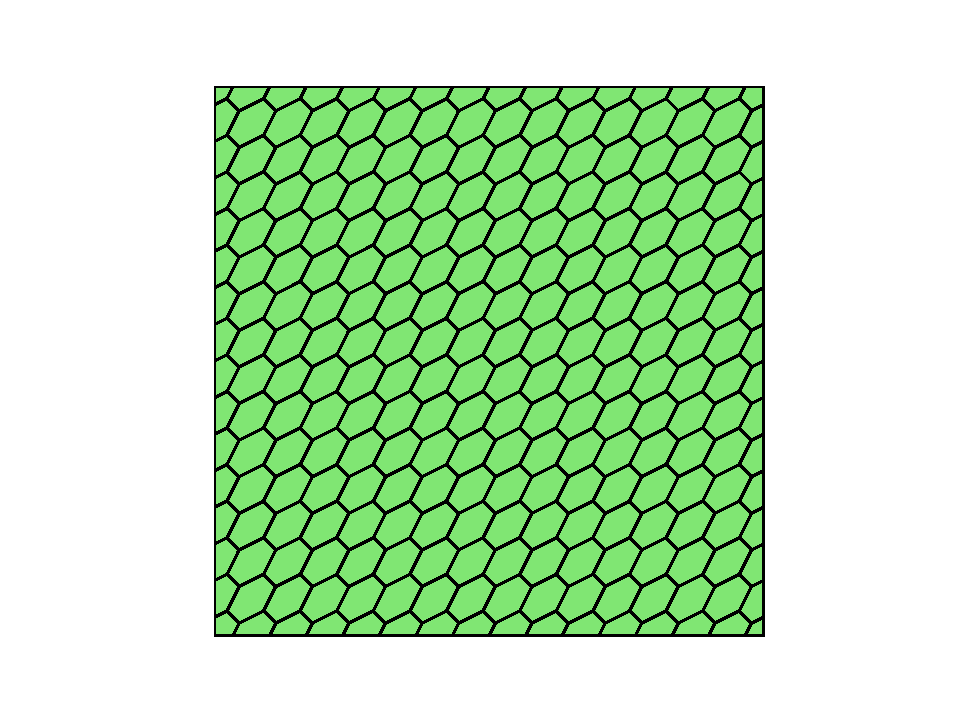
\includegraphics[width=5cm]{./figures/hmvem/convex.pdf}
\end{minipage}%
\begin{minipage}[t]{0.49\linewidth}
\centering
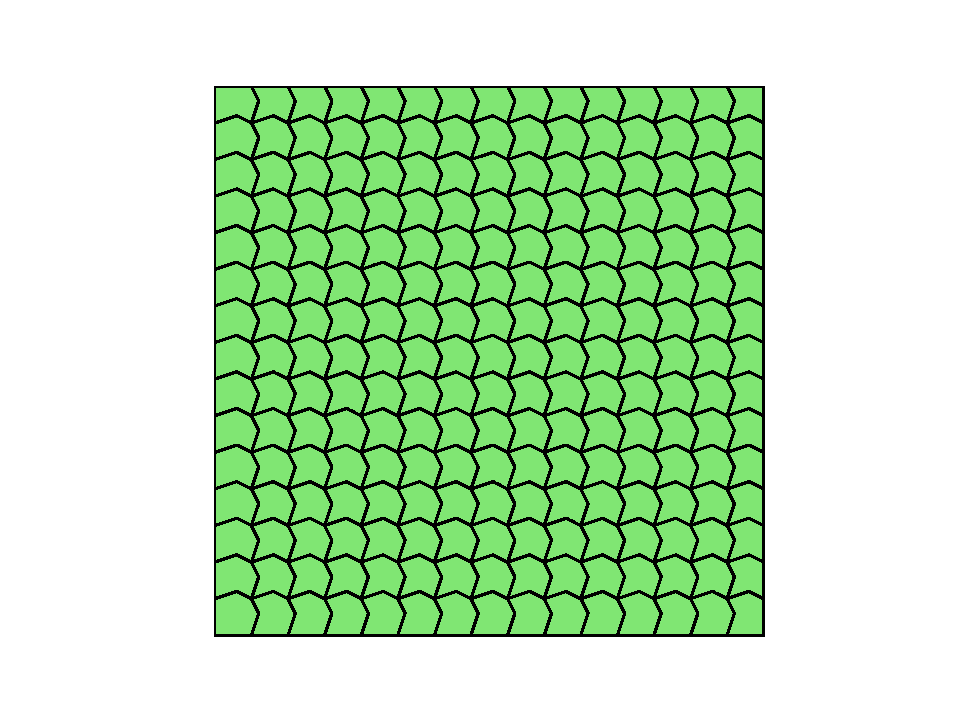
\includegraphics[width=5cm]{./figures/hmvem/nonconvex.pdf}
\end{minipage}%
\centering
\caption{凸多边形网格 $\mathcal{T}_0$(左)与非凸多边形网格
$\mathcal{T}_1$(右).}
\label{fig:mesh}
\end{figure}

\begin{example}\label{exam1}
考虑 $m=2$ 的多重调和方程 \eqref{eq:polyharmonic},其精确解设为 $u = \sin^2(\pi x)\sin^2(\pi y)$,右端项 $f$ 由方程 \eqref{eq:polyharmonic} 计算得到。
\end{example}

选择 $k = 2, 3, 4, 5$ 进行虚单元方法 \eqref{Hmcfmvem} 计算,数值结果如图
 \ref{fig:H2error_convex} 和 图\ref{fig:H2error_nonconvex} 所示。
从图中可知,$|u - \Pi_h u_h|_{2, h} = O(h^{k-1})$,与定理 \ref{errorestimate} 的理论收敛阶相符。

% 第一个图(左半部分:凸多边形网格)
\begin{figure}[htbp]
\centering
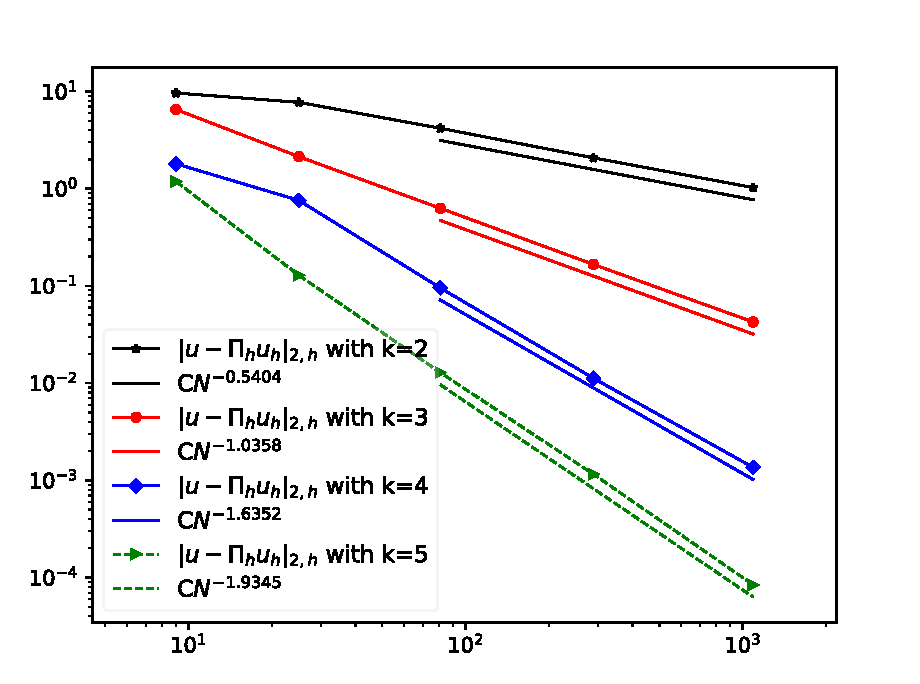
\includegraphics[width=10cm]{./figures/hmvem/H2_convex.pdf}
\caption{算例 \ref{exam1}在凸多边形网格 $\mathcal{T}_0$ 上的误差 $|u - \Pi_h u_h|_{2, h}$,$k = 2, 3, 4, 5$.}
\label{fig:H2error_convex}
\end{figure}

% 第二个图(右半部分:非凸多边形网格)
\begin{figure}[htbp]
\centering
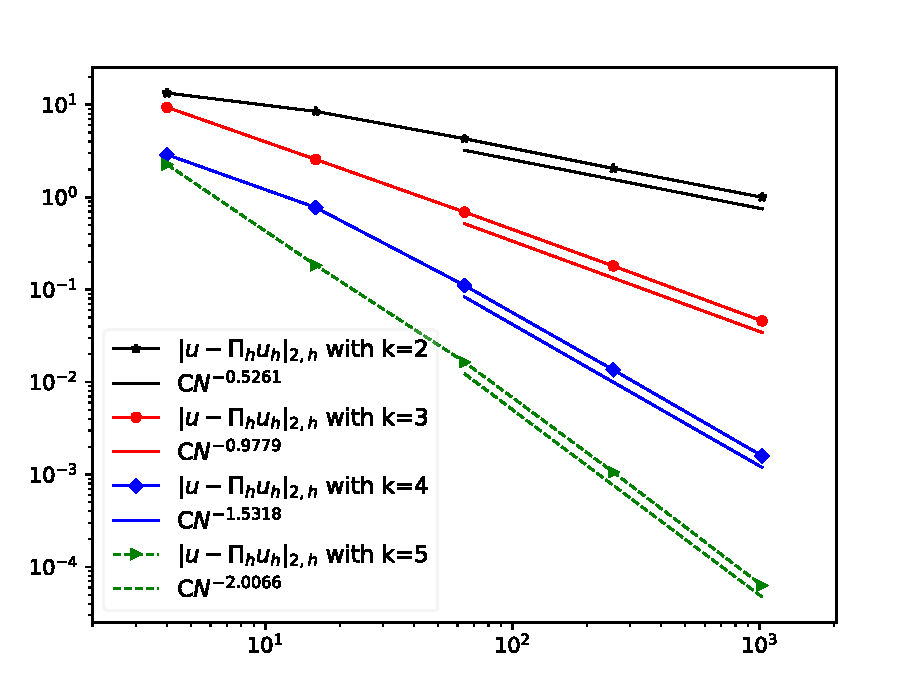
\includegraphics[width=10cm]{./figures/hmvem/H2_nonconvex.pdf}
\caption{算例 \ref{exam1}在非凸多边形网格 $\mathcal{T}_1$ 上的误差 $|u - \Pi_h u_h|_{2, h}$,$k = 2, 3, 4, 5$.}
\label{fig:H2error_nonconvex}
\end{figure}
\begin{example}\label{exam2}
考虑 $m=3$ 的多重调和方程 \eqref{eq:polyharmonic},其精确解设为 $u = \sin^3(\pi x)\sin^3(\pi y)$,右端项 $f$ 由方程 \eqref{eq:polyharmonic} 计算得到。
\end{example}

本算例取 $k = 3, 4, 5, 6$,数值结果如图 \ref{fig:H3error_convex} 和图
\ref{fig:H3error_nonconvex} 所示,
从图中可知 $|u - \Pi_h u_h|_{3, h} = O(h^{k-2})$,与定理 \ref{errorestimate} 的理论收敛阶一致。

% 第一个图(左半部分:凸多边形网格)
\begin{figure}[htbp]
\centering
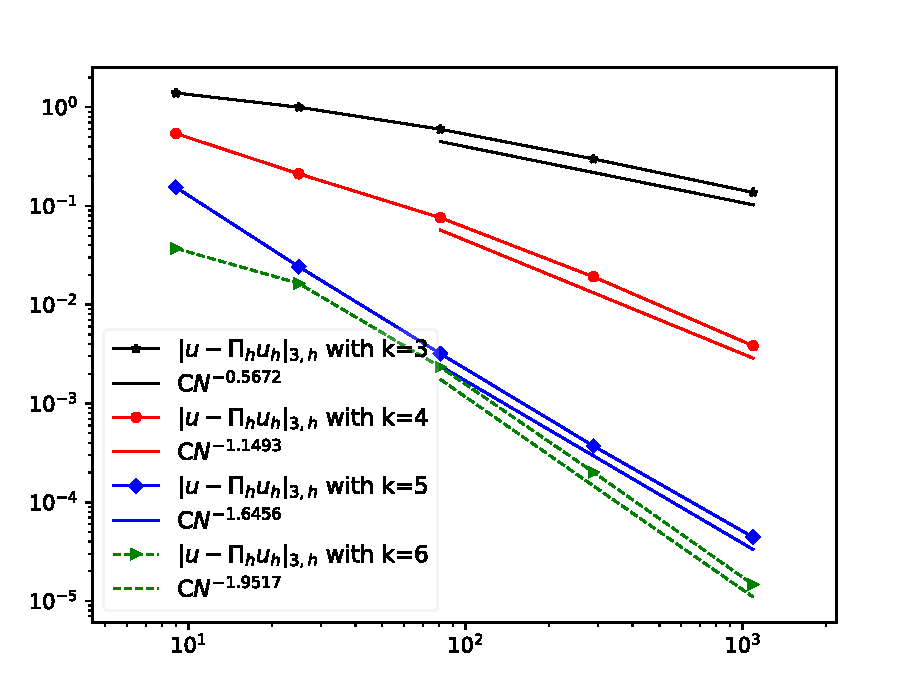
\includegraphics[width=10cm]{./figures/hmvem/H3_convex.pdf}
\caption{算例 \ref{exam2} 在凸多边形网格 $\mathcal{T}_0$ 上的误差 $|u - \Pi_h u_h|_{2, h}$,$k = 2, 3, 4, 5$.}
\label{fig:H3error_convex}
\end{figure}

% 第二个图(右半部分:非凸多边形网格)
\begin{figure}[H]
\centering
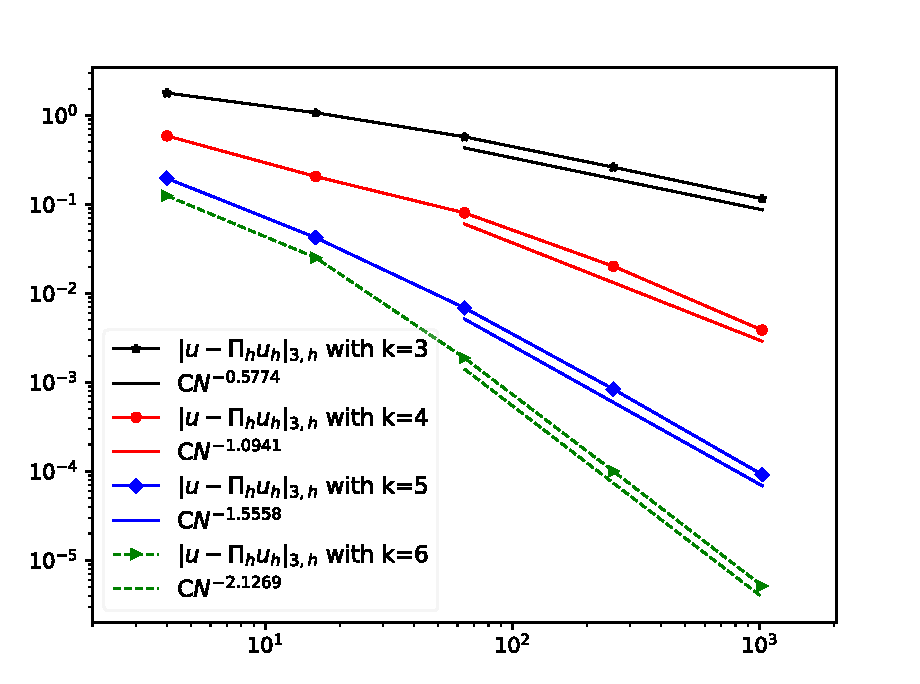
\includegraphics[width=10cm]{./figures/hmvem/H3_nonconvex.pdf}
\caption{算例 \ref{exam2} 在非凸多边形网格 $\mathcal{T}_1$ 上的误差 $|u - \Pi_h u_h|_{2, h}$,$k = 2, 3, 4, 5$.}
\label{fig:H3error_nonconvex}
\end{figure}
